\documentclass[pdflatex,sn-basic]{sn-jnl}

\usepackage{amsmath,amssymb}
\usepackage{bm}
\usepackage{graphicx}
\usepackage{booktabs}
\usepackage{array}
\usepackage{textcomp}
\usepackage{xcolor}
\usepackage{manyfoot}
\usepackage[section]{placeins}

\raggedbottom

\begin{document}

\title[Conservative DBS Formulation for PHREEQC-Coupled Reactive Transport]{A Conservative Darcy-Brinkman-Stokes Formulation for PHREEQC-Coupled Reactive Transport with Cell-Based Surface Complexation}

\author*[1,2]{\fnm{Hannah P.} \sur{Menke}}\email{H.Menke@hw.ac.uk}

\author[1,2]{\fnm{Florian} \sur{Doster}}

\author[1,2]{\fnm{Julien} \sur{Maes}}

\affil*[1]{\orgdiv{Institute for GeoEnergy Engineering}, \orgname{Heriot-Watt University}, \orgaddress{\city{Edinburgh}, \country{United Kingdom}}}

\affil[2]{\orgdiv{SET-IT (Subsurface Energy Transition \& Innovation Centre)}, \orgname{Heriot-Watt University}, \orgaddress{\city{Edinburgh}, \state{Scotland}, \country{United Kingdom}}}

\abstract{We present a conservative Darcy-Brinkman-Stokes (DBS) formulation for
PHREEQC-coupled reactive transport with cell-based surface complexation in
image-based porous media. Implemented in the OpenFOAM-based GeoChemFoam
framework, the formulation transports dissolved species in the physical
mobile-water fraction, stores adsorbed species as conservative cell-scale
surface inventories, and couples each reactive cell to PHREEQC. Reactive
surface area is supplied independently as a cell field, allowing unresolved
internal area in segmented microporous phases to be represented while DBS flow
and transport are retained in resolved pore space.

The implementation is assessed through tests that separate conservative
transport--chemistry coupling from surface-area construction. A one-dimensional
analytical retardation benchmark and closed-system batch tests evaluate the
aqueous and adsorbed mass balance. Controlled two- and three-dimensional
geometries test the smooth-interface surface-area algorithms, while image-based
fracture-network and Estaillades limestone cases examine reactive transport in
heterogeneous pore structures.

The application set spans Pb$^{2+}$ retardation by hydrous ferric oxide
coatings in a two-dimensional fracture network, competitive Mn$^{2+}$/Mg$^{2+}$
exchange in a three-dimensional Kelvin-cell sorbent geometry, and
Sr$^{2+}$/Ca$^{2+}$ exchange in Estaillades limestone. The fracture-network and
limestone cases illustrate how the formulation produces spatially resolved
aqueous and adsorbed
inventories when reactive surface area is partly unresolved at the image scale.
The resulting framework supports conservative surface-complexation modelling
across resolved and unresolved pore structures relevant to contaminant
retention, selective ion capture, and radionuclide transport.}


\keywords{Darcy-Brinkman-Stokes, PHREEQC, surface complexation, micro-continuum reactive transport, image-based porous media, direct lithium extraction}

\maketitle

\begingroup
\centering\fontsize{4.5}{5.5}\selectfont
\textbf{ORCID iDs:} Hannah P. Menke \href{https://orcid.org/0000-0002-1445-6354}{0000-0002-1445-6354};
Florian Doster \href{https://orcid.org/0000-0001-7460-573X}{0000-0001-7460-573X};
Julien Maes \href{https://orcid.org/0000-0002-3248-9758}{0000-0002-3248-9758}\par
\endgroup

\noindent\textbf{Article Highlights}
\begin{itemize}
\item One-dimensional tests reproduce delayed solute transport while tracking dissolved and surface-bound mass.
\item Image-based tests assess how reactive surface area is represented in two and three dimensions.
\item The cell field accounts for reactive area that is unresolved at the image scale.
\end{itemize}

\section{Introduction}

Chemical exchange between the flowing aqueous phase and the solid matrix
governs the transport of dissolved species in porous media alongside advection
and diffusion. In many subsurface systems this exchange proceeds by surface
complexation, ion adsorption, and fast local equilibrium reactions, which
retard dissolved species, reshape concentration fronts, and alter the apparent
accessibility of pore space \citep{dzombak1990surface}. The effects are
strongest in multi-scale rocks that combine open macropores with microporous
matrix regions, where a single image may contain fast transport pathways, slow
exchange domains, and a large internal reactive area that the image cannot
resolve \citep{menke2021upscaling}. The same physics governs contaminant
retention and acid mine drainage treatment
\citep{webster1998trace,blowes2000treatment}, critical-mineral recovery and
direct lithium extraction \citep{reich2022lithium,vera2023environmental}, and
radionuclide transport for geological disposal
\citep{miller2010upscaling,dewindt2019reactive,bildstein2019rtm}, in all of
which selective adsorption or ion exchange may be controlled by surface area
that is not resolved at the image scale.

Three classes of model are available, and each is limited in a different way.
Classical Darcy-scale reactive transport models represent adsorption and
surface complexation through effective source terms, bulk sorption
coefficients, or equilibrium closures applied to the continuum volume
\citep{steefel1990kinetic,steefel1994coupled,steefel2015reactive,mayer2002multicomponent,xu2006toughreact,lichtner1985continuum}.
They remain indispensable for large-domain prediction, but they require
constitutive upscaling assumptions for both transport and reactive surface
area, and they cannot reproduce the spatial heterogeneity of surface inventory
that image-based data make visible \citep{battiato2011applicability}. Fully
resolved pore-scale models, including direct numerical simulation
\citep{molins2021simulation,molins2015reactive,molins2012investigation,starchenko2018development},
lattice Boltzmann methods \citep{yoon2015lattice,kang2007lattice}, and
explicit-boundary DBS approaches
\citep{maes2018direct,maes2021geochemfoam,soulaine2017mineral}, instead locate
reactive uptake at the meshed grain surface. This is appropriate when the
dominant surface area coincides with the resolved interface between pore and
grain, but it is bounded by image resolution: once internal micro-scale area
falls below the mesh scale, a boundary-resolved description is no longer
faithful to the physical geometry, and the cost of resolving it rises steeply.
Pore-network and other reduced pore-scale models occupy a middle ground
\citep{blunt2001flow}, but they depend on idealised throat-and-pore
representations and do not deliver the voxel-by-voxel field description used in
image-based DBS simulations.

The consequences are specific in image-based simulations of carbonate and other
multi-scale porous media \citep{menke2015dynamic, menke2018fourd,
menke2021upscaling,wildenschild2013xray,blunt2013porescale}. Segmented images
routinely separate macropore, microporous, and nearly solid regions, but the
reactive internal surface of the microporous phase is not the same object as
the explicitly meshed boundary of the coarse computational cells. Ignoring that
internal area under-predicts reactive uptake. Inserting it as an ad hoc
volumetric sink leaves both the conservation properties and the meaning of the
cell-scale surface inventory unclear.

PHREEQC and its reaction-module form, PhreeqcRM, already provide the required
chemistry: aqueous speciation, surface complexation, equilibrium and kinetic
reactions, and operator-split coupling to transport simulators
\citep{parkhurst2013phreeqc, parkhurst2015phreeqcrm,charlton2011modules}.
Existing PHREEQC-coupled workflows serve structured-grid continuum models and
operator-split multi-component solvers well \citep{jyoti2021validation}. The
open question is how to embed that engine in a transport formulation consistent
with unresolved image-based geometry. The closest existing approach is
\texttt{porousMedia4Foam} \citep{soulaine2021porousmedia4foam,
pavuluri2022reactive}, which couples a micro-continuum OpenFOAM solver to
PHREEQC at pore, hybrid, and Darcy scales, but which applies chemistry through
kinetic or equilibrium flux conditions at the diffuse fluid-solid interface. It
therefore inherits the limitation of the fully resolved methods, in that the
reactive surface must overlap the resolved computational boundary, and it draws
no explicit distinction between the numerical DBS porosity used to regularize
transport and the physical mobile-water fraction that governs chemistry.
Earlier PHREEQC-coupled cases within GeoChemFoam itself
\citep{maes2022heat,maes2022vos} share this restriction: they support reactive
transport and surface complexation where the reactive surface coincides with an
explicit mesh boundary, which remains valid but does not cover the case in
which the dominant reactive area lies inside the coarse cell.

In this work we develop a DBS-compatible reactive transport formulation in
which the reactive surface is a property of the cell rather than of the mesh
boundary. Aqueous transport is written for the physical mobile-water fraction;
unresolved reactive surface area is prescribed as a cell field and carried as a
cell-centred adsorbed inventory; local PHREEQC chemistry transfers mass
conservatively between the aqueous and adsorbed states; and no heuristic
redistribution of source terms is used. Two consequences follow. The
formulation requires an explicit separation between the numerical DBS porosity
that stabilizes transport in nearly solid voxels \citep{soulaine2016micro} and
the physical mobile-water fraction that sets chemical concentrations. It also
requires the surface inventory to be defined at cell centres and driven by an
unresolved internal surface-area density, rather than reconstructed on mesh
faces. Together these choices let the method act on microporous matrix regions
instead of only on explicitly resolved boundaries between pore and grain. The
governing equations are posed on general finite-volume meshes; the image-based
cases used here are the motivating application.

The solver that results, \texttt{reactiveTransportDBSFoam}, couples
conservative DBS transport to PHREEQC-based surface complexation at the cell
scale. A one-dimensional analytical retardation solution provides a closed-form
reference for the coupled advection, diffusion and sorption system, and
closed-system batch calculations test the aqueous and adsorbed mass balance.
The surface-area algorithms are verified on controlled geometries of known area
and on image-based micromodels, and a resolved-to-DBS two-scale benchmark of
selective Li$^{+}$ uptake tests whether the upscaled cell-based description
reproduces a fully resolved calculation of the same system. The formulation is
then applied to three image-based geometries of increasing complexity:
Pb$^{2+}$ uptake on hydrous ferric oxide (HFO) in a two-dimensional fracture
network, as an analogue for heavy-metal remediation in fractured aquifers and
permeable reactive barriers; selective Mn$^{2+}$ uptake from a Mg$^{2+}$-rich
brine on HFO in a three-dimensional Kelvin-cell sorbent, as an analogue for
critical-metal capture; and Sr$^{2+}$ migration in Estaillades limestone, as an
analogue for radionuclide transport in a deep geological repository (DGR).
Together these cases determine how resolved pore geometry and unresolved
internal surface area interact to control the spatial distribution of aqueous
and adsorbed species in multi-scale porous media.

\section{Model Description}
\label{sec:model}

\subsection{Field Definitions}

The DBS micro-continuum formulation \citep{brinkman1949calculation,soulaine2016micro,
soulaine2024microcontinuum} represents the pore medium as a continuum in which
a cell-centred porosity field $\epsilon$ varies smoothly from
zero (solid) to unity (open pore). The steady incompressible flow is governed
by the Darcy--Brinkman equations:
\begin{align}
\nabla \cdot \bm{u}_D &= 0,
\label{eq:continuity} \\
-\nabla p + \nabla \cdot \bigl(\mu_{\mathrm{eff}} \nabla \bm{u}\bigr)
- \frac{\mu}{K(\epsilon)}\,\bm{u}_D &= \bm{0},
\label{eq:brinkman}
\end{align}
where $\bm{u}_D = \epsilon\bm{u}$ is the Darcy velocity,
$\mu$ is the fluid viscosity, $\mu_{\mathrm{eff}}$ is an effective
viscosity that smoothly recovers the Stokes equation in open-pore cells
\citep{soulaine2016micro}, and $K(\epsilon)$ is a permeability
function. The drag coefficient $\mu/K(\epsilon)$ therefore acts
as a large resistance term in solid-like cells and vanishes in open-pore cells,
so Eq.~\eqref{eq:brinkman} reduces to the Stokes equation.

The reactive-transport model uses two cell-centred material fields. The
porosity $\epsilon$ is the mobile-water volume per bulk cell volume and enters
both DBS transport and the fixed PHREEQC cell mapping. In the analytical
derivations below it is denoted $\theta$ to retain the conventional notation
for mobile-water fraction; thus $\theta=\epsilon$ in every reported case. The
second field is the reactive internal surface area per bulk volume $a_{\mathrm{surf}}$
(m$^2$\,m$^{-3}$), which represents surface available for adsorption and
surface complexation. All aqueous species, together with $\epsilon$,
$a_{\mathrm{surf}}$, and the adsorbed surface fields, are cell-centred; the
transport flux is evaluated on cell faces.

\subsection{Reactive Surface Area Field}
\label{sec:aSurf}

The DBS micro-continuum framework naturally produces three distinct local
material states within a computational cell: a resolved macro-pore (high
$\theta$, negligible grain fraction), a microporous grain (intermediate
$\theta$, significant unresolved grain fraction), and a near-solid or
fully solid region (very low $\theta$). All three must contribute reactive
surface area to the chemistry, but they do so through different geometric
mechanisms. Both contributions are captured in the single cell-centred field
$a_{\mathrm{surf}}$ (units: m$^2\,\mathrm{m}^{-3}_{\mathrm{bulk}}$), which is
the sum of two terms:
\begin{equation}
a_{\mathrm{surf}} = a_{\mathrm{surf}}^{\mathrm{interface}} +
a_{\mathrm{surf}}^{\mathrm{intrinsic}}.
\label{eq:asurf}
\end{equation}

The first term, $a_{\mathrm{surf}}^{\mathrm{interface}}$, is computed
geometrically from the segmented voxel image. The user designates one image
label as the \emph{reference grain phase}; this is simply the segmented label
whose visible image-scale boundary is counted as reactive interface. It may
correspond to a microporous grain, a dense solid, or any other label assigned
to the reactive surface. In general,
$a_{\mathrm{surf}}^{\mathrm{interface}}$ is the local interface area per bulk
cell volume obtained by reconstructing the boundary of that reference phase
inside each finite-volume cell.

The interface contribution is obtained by reconstructing a sub-voxel boundary from the
same segmented image before accumulating area back into the computational
fluid dynamics (CFD) cells. The segmented owner phase is converted to a smoothed
occupancy field, a sub-voxel interface is extracted, and the resulting line or
surface measure is assigned to the owning finite-volume cells as a bulk
$a_{\mathrm{surf}}$ field.
Section~\ref{sec:valSummary} validates this geometric construction separately
from the intrinsic micropore contribution. The resulting total field is
supplied explicitly to the reactive-transport solver.

The interface term captures only grain--fluid boundaries that are visible at
the resolved image scale. It does not detect
reactive area that lies entirely \emph{within} a voxel, such as sub-voxel
surface roughness of a grain or the internal pore network of a microporous
phase. Those surfaces are below the image resolution by construction.

The second term, $a_{\mathrm{surf}}^{\mathrm{intrinsic}}$, accounts for this
sub-voxel contribution. A volumetric surface density $s_k$
(units: m$^2$\,m$^{-3}$) is prescribed for each segmented image label $k$
(for example pore, micropore, or dense solid); it may
represent any sub-voxel surface that the image cannot resolve --- for example
the Brunauer--Emmett--Teller (BET) surface area of a microporous grain measured
by N$_2$ adsorption, or the surface roughness of a dense solid grain measured
on powdered material.
The intrinsic contribution is assembled by weighting each phase density by
its local volume fraction $f_k$ within the coarse cell:
\begin{equation}
a_{\mathrm{surf}}^{\mathrm{intrinsic}} = \sum_k f_k\,s_k.
\label{eq:asurf_intrinsic}
\end{equation}
$s_k$ may be non-zero for any label, including the reference grain phase
itself. The same segmented label may contribute through both terms:
$a_{\mathrm{surf}}^{\mathrm{interface}}$ gives the image-scale outer surface
of the grain, and $a_{\mathrm{surf}}^{\mathrm{intrinsic}}$ adds the
sub-voxel surface area that the image resolution cannot capture. If
$s_k = 0$ for all labels, the total reduces to the purely geometric
image-scale surface. Both contributions are pre-computed from the segmented image
before the flow simulation begins and are held constant throughout the
reactive-transport calculation.

Both contributions enter the geochemical module in the same way. The
PhreeqcRM surface convention used here is based on representative bulk volume.
The volumetric area field is therefore converted only from cubic metres to
litres:
\begin{equation}
a_{\mathrm{surf}}^{\mathrm{bulk,L}} = \frac{a_{\mathrm{surf}}}{10^{3}},
\label{eq:asurf_bulk_litre}
\end{equation}
where the factor $10^3$ converts cubic metres to litres. Surface areas
estimated from nano-computed tomography
(nano-CT), micro-computed tomography (micro-CT), focused ion beam scanning
electron microscopy (FIB-SEM), or other image data are first expressed on a
bulk-volume basis (m$^2$\,m$^{-3}_{\mathrm{bulk}}$), consistent with
Eqs.~\eqref{eq:asurf}--\eqref{eq:asurf_intrinsic}. Image-derived surface areas
reported per microporous-phase volume or per grain mass are converted to this
bulk-volume basis before Eq.~\eqref{eq:asurf_bulk_litre} is applied.

The same fixed porosity field is used for DBS transport and for the PHREEQC
solution volume. Cells in
which $\theta$ falls below the chemistry mask threshold
$\theta_{\mathrm{mask}}$ are treated as chemically inactive and their surface
terms are suppressed.

\subsection{Conservative Aqueous Transport}

For each aqueous species with concentration $C_i$, the conservative DBS
transport equation is written as
\begin{equation}
\frac{\partial (\theta C_i)}{\partial t}
+ \nabla \cdot (\bm{u}_D C_i)
- \nabla \cdot (\theta D_i \nabla C_i) = 0,
\end{equation}
where $\bm{u}_D$ is the Darcy velocity satisfying
Eqs.~\eqref{eq:continuity}--\eqref{eq:brinkman}, and $D_i$ denotes the
diffusivity used in the transport equation. In fully resolved macro-pore cells
($\theta \approx 1$), $D_i$ is the free molecular diffusivity. In cells that
represent microporous material ($0 < \theta < 1$), $D_i$ is interpreted as an
effective diffusivity, commonly $D_i = D_i^{\mathrm{mol}}/\tau$, where
$D_i^{\mathrm{mol}}$ is the molecular diffusivity and $\tau \geq 1$ is the
tortuosity factor of the micropore network. In either case, the $\theta$ factor
multiplying $D_i$ in the diffusion term already accounts for the reduced
water volume available for transport. There is no chemistry source term in
this equation: reactions are handled by the subsequent operator-split
PHREEQC step and do not appear as an explicit right-hand side here.

In the implementation, $\theta$ in this equation is the OpenFOAM field
\texttt{eps}; this field is fixed during all PHREEQC calculations reported here.

For a vector of aqueous species $\bm{C}$, the same transport balance can be
written in
compact form as
\begin{equation}
\frac{\partial (\theta \bm{C})}{\partial t}
+ \nabla \cdot (\bm{u}_D \bm{C})
- \nabla \cdot (\theta \bm{D} \nabla \bm{C}) = \bm{0},
\end{equation}
which makes the conservative structure explicit before any chemistry update is
applied.

\subsection{Cell-Based Surface Inventory}

For the cell-based unresolved surface carried by the DBS formulation, the
conservative local inventory is expressed
in the current solver field variables as
\begin{equation}
M = \theta C + a_{\mathrm{surf}}\Gamma,
\label{eq:inventory}
\end{equation}
where $\Gamma$ is the cell-centred surface-species concentration written by
the implementation (mol\,m$^{-2}$ of reactive surface). The first term is the
aqueous amount per bulk volume and the second is the adsorbed amount per bulk
volume. Porosity enters the aqueous inventory exactly once; the bulk-based
surface-area field requires no additional porosity scaling.

This field-level expression is the appropriate quantity for analytical
comparisons and for benchmark inventory checks. For multiple surface species,
the local bulk inventory is obtained by summing the relevant aqueous and
adsorbed contributions. Single-species notation is used below only for clarity;
all reported totals are evaluated in the actual implemented field variables.

\subsection{Local Chemistry Coupling}

The chemical update is local to each cell. Over one transport--chemistry
cycle, the transport step first advances the aqueous species in conservative
finite-volume form. The updated cell state, together with the mobile-water
fraction and cell-based surface state, is then mapped into PHREEQC
\citep{parkhurst2013phreeqc} via the PhreeqcRM interface
\citep{parkhurst2015phreeqcrm}. PHREEQC solves the local chemistry under the
assumption of \emph{thermodynamic equilibrium}: within each timestep, surface
complexation reactions are treated as instantaneous relative to transport.
This is appropriate when the equilibration timescale of the surface reactions
is short compared with the transport timescale. The relevant transport regime
is characterised by the P\'{e}clet number, $Pe = U L / D$, where $U$ is a
representative velocity, $L$ is a representative transport length, and $D$ is
the aqueous diffusion coefficient. This equilibrium assumption holds when
surface equilibration is fast relative to advection and diffusion over the
resolved transport length scale. Kinetic surface reactions can in principle be
handled by the same interface but are not used in the present work.

The solver uses first-order Lie splitting \citep{carrayrou2004operator}. The
splitting introduces a global error of $\mathcal{O}(\Delta t)$ in the
operator-split solution; the local error over one step is
$\mathcal{O}(\Delta t^2)$. For the timesteps used here, the advective
Courant--Friedrichs--Lewy (CFL) number remains $O(1)$, so the
operator-splitting error is of the same formal order as the first-order
transport discretization. The resulting algorithm keeps the conservative
transport update and the local PHREEQC equilibrium update as distinct
operators within each timestep.

At the algorithmic level, one timestep of size $\Delta t$ is:
\begin{align}
\widetilde{\bm{C}}^{\,n+1} &= \mathcal{T}_{\Delta t}(\bm{C}^{n}, \theta, \bm{u}_D, \bm{D}),\\
(\bm{C}^{n+1}, \bm{\Gamma}^{n+1}) &=
\mathcal{R}_{\Delta t}(\widetilde{\bm{C}}^{\,n+1}, \bm{\Gamma}^{n}, \theta, a_{\mathrm{surf}}),
\end{align}
where $\mathcal{T}_{\Delta t}$ is the conservative finite-volume transport
operator (advancing $\theta\bm{C}$ in DBS form) and $\mathcal{R}_{\Delta t}$
is the local PHREEQC equilibrium operator that updates both aqueous and
surface states simultaneously within each cell.

\subsection{Analytical Dilute Limit}

In the dilute linear-equilibrium limit, surface complexation reduces to a
Henry-type isotherm. The standard Henry coefficient is $K_s = \Gamma / C$
(units: m), the ratio of surface concentration $\Gamma$ (mol\,m$^{-2}$) to
aqueous concentration $C$ (mol\,m$^{-3}$):
\begin{equation}
\Gamma = K_s C.
\end{equation}
In practice, $K_s$ is not prescribed directly but is
extracted numerically from a pair of batch equilibrations at two different
aqueous concentrations:
$K_s = \Delta\Gamma / \Delta C$.
This avoids any ambiguity in the PHREEQC database-to-field unit mapping and
provides the coefficient that enters the retardation formula directly.

Substituting into the inventory Eq.~\eqref{eq:inventory} and taking the
time derivative yields the retarded 1D transport equation
\begin{equation}
\left(
\theta + a_{\mathrm{surf}}K_s
\right)\frac{\partial C}{\partial t}
+ \frac{\partial (u_D C)}{\partial x} = 0.
\end{equation}
The corresponding retardation factor is
\begin{equation}
R = 1 + \frac{a_{\mathrm{surf}}\,K_s}{\theta},
\label{eq:retardation}
\end{equation}
Both $a_{\mathrm{surf}}$ and $\theta$ can vary spatially, so
Eq.~\eqref{eq:retardation} also gives the local retardation at any point in
a heterogeneous domain. The analytical advection-diffusion profile against
which the numerical results are compared follows \citet{ogata1961solution},
with the advection velocity $u_D/\theta$ replaced by $u_D/(\theta R)$
and the diffusivity replaced by $D/R$.

\subsection{Validation Requirements}

The validation programme presented in this paper is designed to establish four
criteria. First, the formulation must reduce to simpler known limits. Second,
the local surface-coupled chemistry must conserve the intended field-level
inventory. Third, the formulation must reproduce the dilute analytical
retardation limit. Fourth, the same formulation must remain applicable without
structural change as the application domain expands from 1D benchmarks to 2D
and 3D image-based cases.

\section{Numerical Implementation}

This section describes the discrete fields, the transport--chemistry coupling,
and the per-timestep algorithm used in the reported simulations. The
implementation couples conservative Darcy-Brinkman-Stokes (DBS) transport
with cell-centred PHREEQC chemistry and cell-based surface complexation in a
single operator-split formulation.

\subsection{Field Locations And Discretization}

The discretization used throughout this paper keeps all chemistry-bearing state
cell-centered. The solution species, $\epsilon$ (denoted $\theta$ in the
analytical equations), $a_{\mathrm{surf}}$, and the adsorbed surface-species fields are stored at
cell centres, whereas the Darcy velocity $\bm{u}_D$ is face-centred. Transport
uses face interpolation within the conservative flux assembly, while surface
chemistry is evaluated as a cell-local update. The additive decomposition of
$a_{\mathrm{surf}}$ into interface and intrinsic contributions is defined in
Section~\ref{sec:aSurf}
(Eqs.~\eqref{eq:asurf}--\eqref{eq:asurf_intrinsic}).

All simulations reported here use the following discretization. Time
integration uses the first-order implicit Euler scheme, consistent with the
first-order Lie splitting of the transport and chemistry operators. The
convective term $\nabla\cdot(\bm{u}_D C_i)$ is discretized with the standard
first-order upwind scheme, which is bounded, monotone, and free of spurious oscillations
on the unstructured image-based meshes used here. The diffusive term
$\nabla\cdot(\theta D_i \nabla C_i)$ uses a second-order Gauss linear scheme
with non-orthogonality correction. The combination gives a scheme that is
first-order accurate in both time and space for advection-dominated transport,
consistent with the overall first-order operator-split framework.

\subsection{PHREEQC Coupling}

The PHREEQC coupling is selected with
\texttt{mixtureType phreeqcMixture} in
\texttt{constant/thermoPhysicalProperties}. This mixture wraps the PhreeqcRM
interface \citep{parkhurst2015phreeqcrm}. At
initialisation, each computational cell is registered as a separate PHREEQC
solution. When surface complexation is active, a PHREEQC \texttt{SURFACE}
block is also created for each reactive cell. For surface master $k$, its
capacity per representative bulk volume is
\begin{equation}
q_{\mathrm{sites},k} = s_k \, a_{\mathrm{surf}},
\label{eq:nsites}
\end{equation}
where $s_k$ (mol\,m$^{-2}$) is the user-prescribed site density for surface
master species $k$. This initialises the reactive capacity consistently with
the bulk-based surface-area field. PhreeqcRM is configured with its bulk
representative-volume surface convention, so no additional division by
porosity is applied.
The OpenFOAM dictionary stores $s_k$ in kmol\,m$^{-2}$, following the native
OpenFOAM amount unit; it is therefore multiplied numerically by $10^3$ when
interpreted as mol\,m$^{-2}$. Each surface-master density is supplied as an
OpenFOAM field, allowing spatially heterogeneous site densities.

The total $a_{\mathrm{surf}}$ field is computed before the simulation begins
(Section~\ref{sec:aSurf}), written as an OpenFOAM volume field, and read
explicitly by \texttt{reactiveTransportDBSFoam}. It is held constant throughout
the reactive-transport calculation; it is not updated by the flow or chemistry
solvers. The area and site capacity are transferred when the per-cell
PHREEQC surface templates are created and remain internal to PhreeqcRM during
the time loop. Consequently, the present implementation supports spatially
heterogeneous but time-independent $\epsilon$ and $a_{\mathrm{surf}}$; changing
either field during reactive transport would require rebuilding the PHREEQC
surface state. The surface mode is optional and reduces exactly to
aqueous-only mode when $a_{\mathrm{surf}} = 0$ everywhere.
For the image-based cases in this paper, a smooth sub-voxel reconstruction is
applied to the segmented occupancy field and the reconstructed
interface back into the CFD cells as volumetric $a_{\mathrm{surf}}$. In three
dimensions, \texttt{smoothSurface} extracts an isosurface and deposits the
resulting triangle areas into the cells that carry the reactive surface. In
quasi-two-dimensional image cases, it extracts an isoline on the image plane,
multiplies the reconstructed line length by the physical out-of-plane
thickness, and assigns the resulting area to the corresponding DBS cells. The
2D and 3D variants produce the same bulk field type and enter the same
cell-local PHREEQC mapping.

Cells with negligible mobile-water fraction
($\epsilon < \texttt{epsChemistryMin}$) are excluded from the fixed
finite-volume-to-PhreeqcRM mapping and do not contribute to chemistry.

The cell-local nature of the chemistry step means that all PHREEQC calls are
embarrassingly parallel across cells. PhreeqcRM distributes the cell
chemistry over available threads using OpenMP, so the chemistry cost scales
with the number of cores used for the transport solve.

\subsection{Per-Timestep Algorithm}

At startup, \texttt{reactiveTransportDBSFoam} reads the fixed porosity,
velocity, pressure, species, and explicit total surface-area fields. The
\texttt{phreeqcMixture} constructor then establishes a fixed mapping between
active finite-volume cells and PhreeqcRM cells. At each timestep, each aqueous
transport equation is advanced in conservative DBS form using the implicit
Euler--upwind discretization described above. The updated aqueous
concentrations and surface states are then pushed into PhreeqcRM, the local
equilibrium chemistry is evaluated for all active cells, and the updated
aqueous and surface concentrations are returned to the finite-volume fields.
The porosity and flow fields are not advanced in this PHREEQC mode. At
configured output times, OpenFOAM fields and a matching PhreeqcRM checkpoint
pair are written for chemically consistent restarts. Conservation is assessed
from the written fields using the domain-integrated bulk inventory
$M_{\mathrm{total}} = \sum_{\mathrm{cells}} V_{\mathrm{cell}}
\left( \theta C + a_{\mathrm{surf}}\Gamma \right)$
as a conservation diagnostic, where $V_{\mathrm{cell}}$ is the cell volume. In
a closed domain this quantity should remain constant to within discretisation
error; in a flow-through domain it should balance the net flux through the
inlet and outlet faces.

The operator-split structure keeps
transport and chemistry individually testable and ensures that the
conservative structure of the aqueous transport step is not hidden inside a
composite implicit source term.

\begin{figure}[htbp]
    \centering
    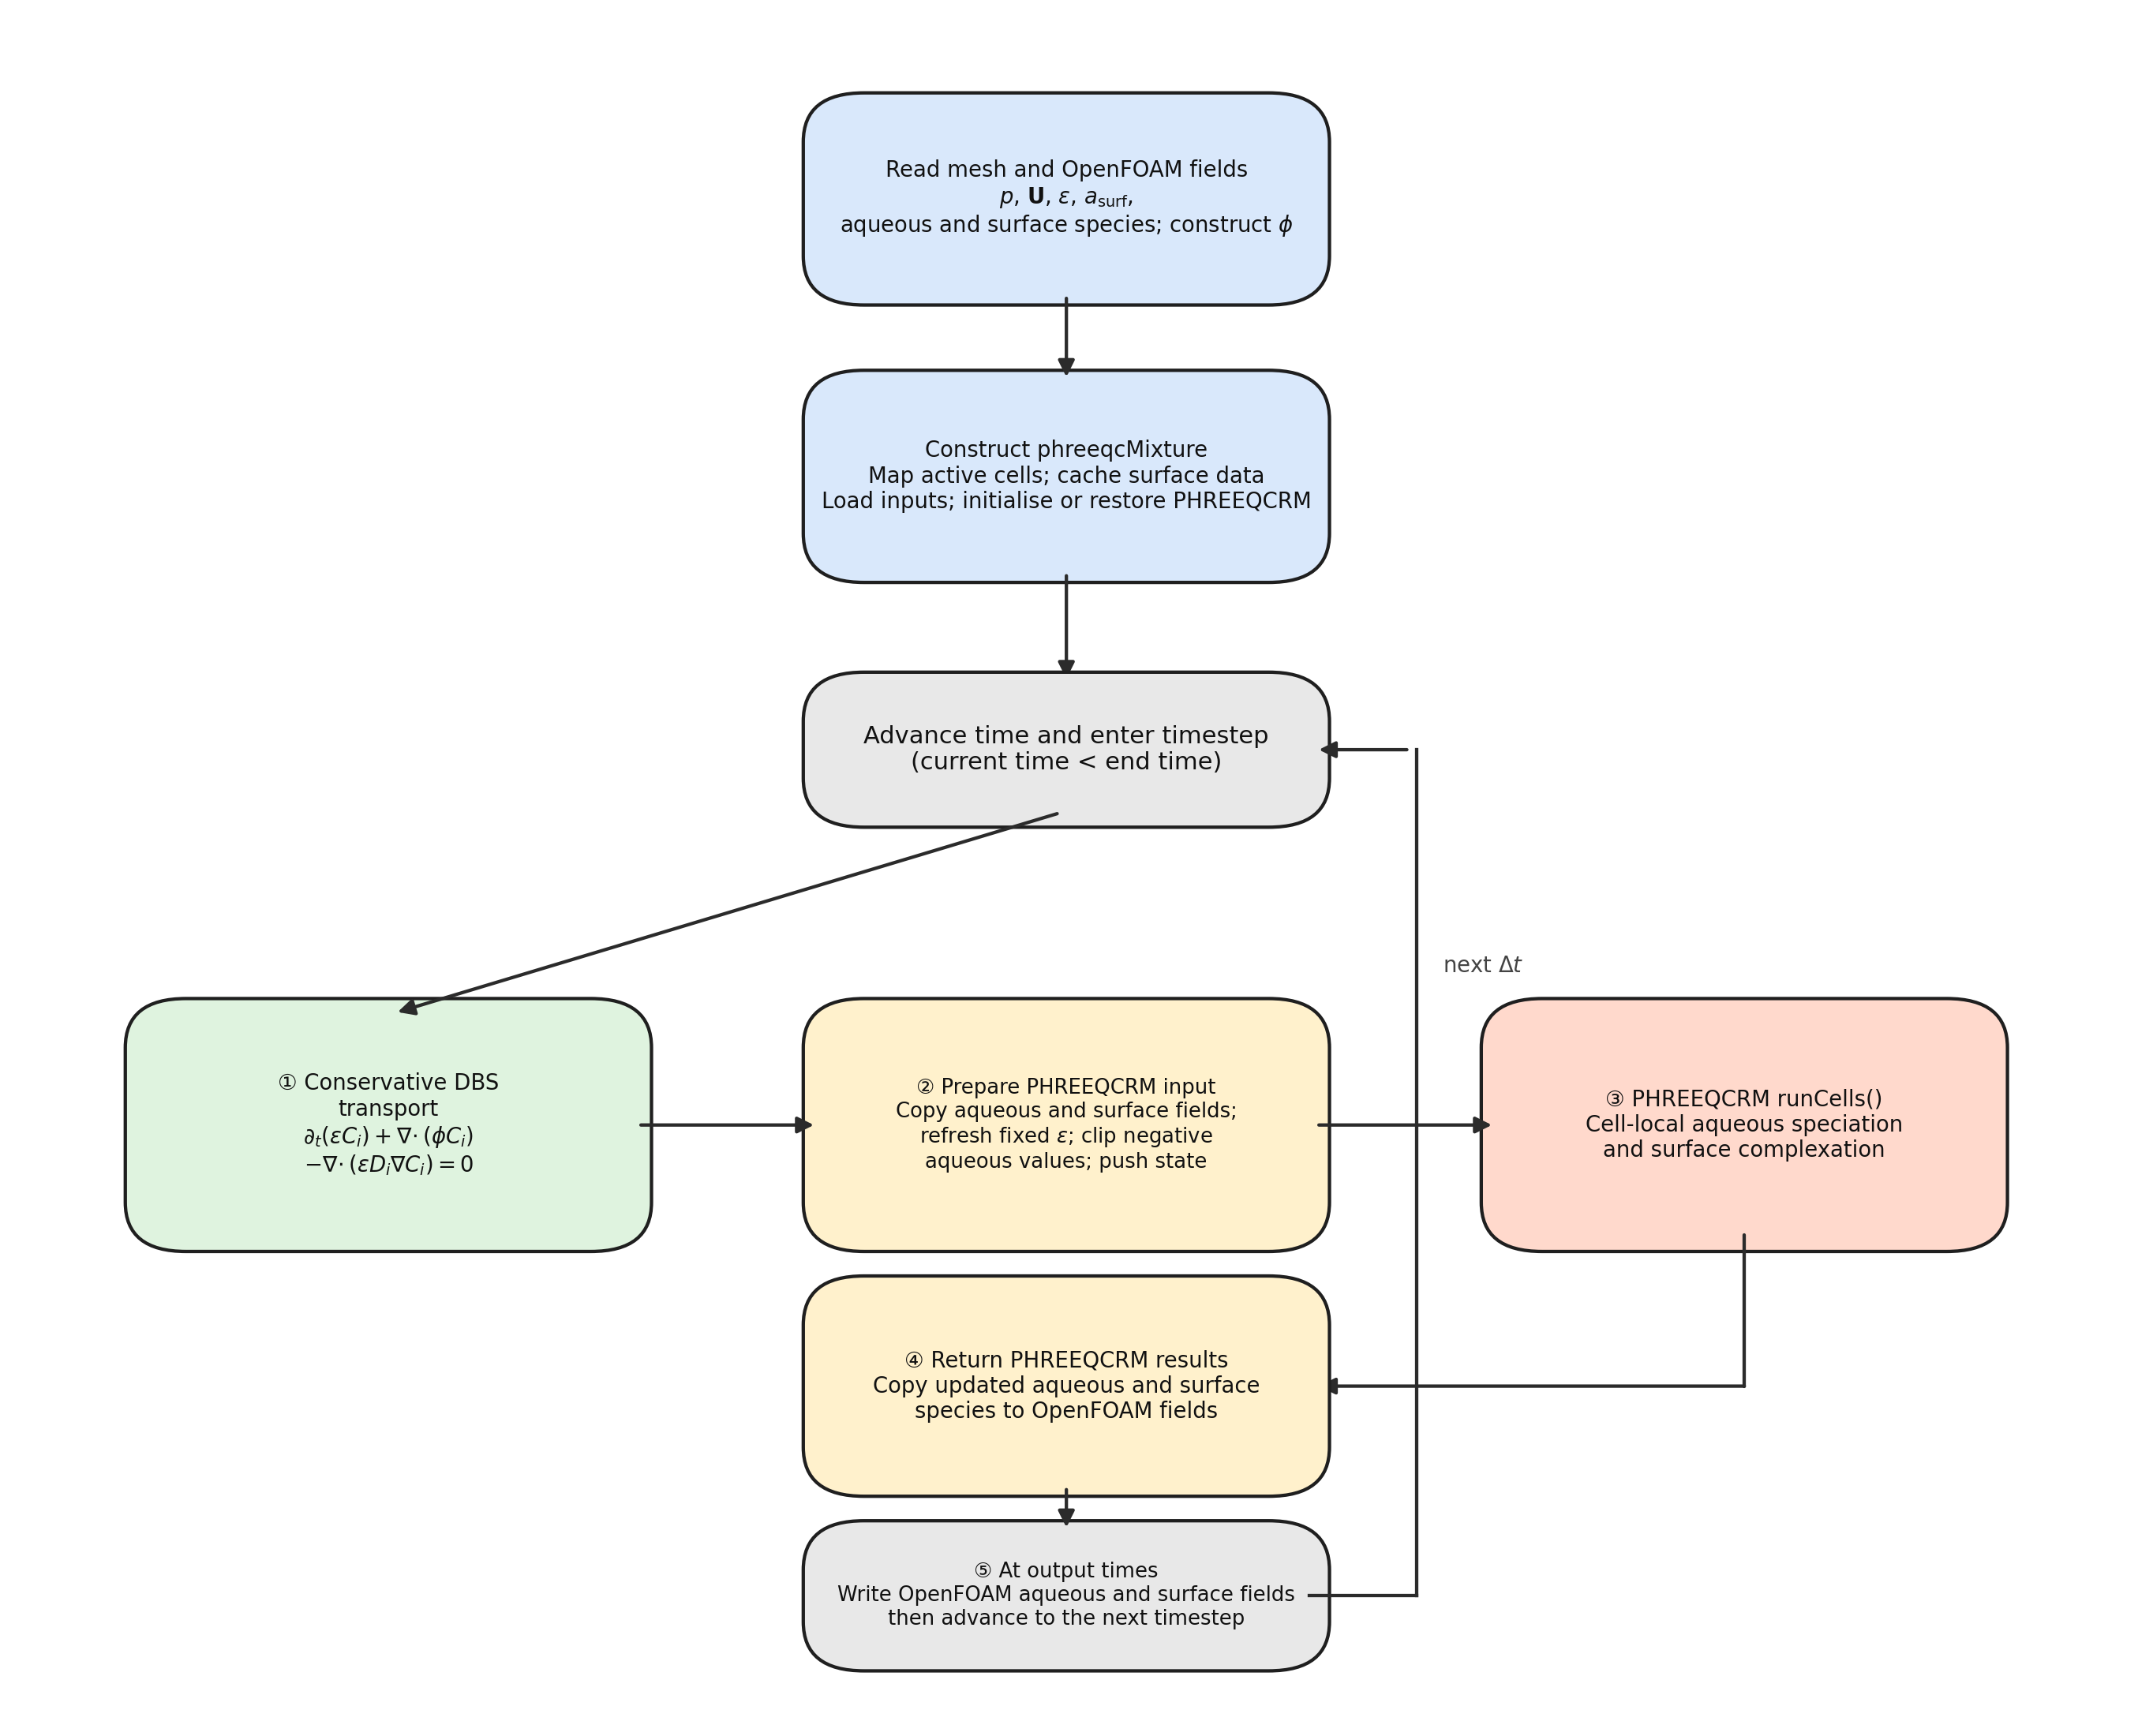
\includegraphics[width=0.96\linewidth]{figures/png/fig05_solver_workflow.png}
    \caption{Full solution procedure for
    \texttt{reactiveTransportDBSFoam}. The solver reads the current
    finite-volume state, initializes or updates the cell-based PHREEQC
    coupling through \texttt{phreeqcMixture}, advances all aqueous species
    in conservative DBS form, executes the local cellwise chemistry update,
    and then writes the updated aqueous and surface states back to the
    finite-volume fields. The workflow is intentionally operator-split:
    transport is solved first, followed by local PHREEQC chemistry, so the two
    operators remain independently testable and the conservative structure of
    the aqueous transport step is never hidden inside an implicit composite
    source term.}
    \label{fig:dbsWorkflow}
\end{figure}

Figure~\ref{fig:dbsWorkflow} illustrates the implemented algorithm. Solver
selection is made through \texttt{mixtureType}: the surface-complexation cases
use \texttt{phreeqcMixture}, whereas the upstream kinetic-mineral formulation
uses \texttt{inertMultiComponentMixture}. The chemistry state remains
cell-centred throughout the loop. The solver does not
convert the unresolved surface reaction into an equivalent face flux. Instead,
transport acts through the aqueous face fluxes, while PHREEQC updates the
cell-local aqueous and adsorbed inventories after each transport solve.

\section{Validation}

\subsection{1D Analytical Retardation Benchmark}\label{sec:1D}

The 1D linear-retardation benchmark tests the surface-chemistry coupling on a
uniform domain where the retardation factor has an exact analytical form.
With uniform porosity $\theta$ and surface-area density $a_{\mathrm{surf}}$,
the field-level retardation coefficient is
$R_{\mathrm{field}} = 1 + a_{\mathrm{surf}} K_{s,\mathrm{field}} / \theta^2$,
and the retarded concentration front satisfies the standard advection--diffusion
equation with effective velocity $u / (\theta R_{\mathrm{field}})$ and effective
diffusivity $D / R_{\mathrm{field}}$.
This configuration therefore isolates three coupled components of the
implementation: the batch-secant calibration of $K_{s,\mathrm{field}}$, the
field-level averaging of the surface-capacity term, and the advective--diffusive
transport step. The benchmark compares a surface-enabled transport case, a
matched aqueous-only case (\mbox{$a_{\mathrm{surf}} = 0$}), and a dilute batch
pair used to estimate $K_{s,\mathrm{field}}$ via the secant method.

For the validated benchmark reported here,
$K_{s,\mathrm{field}} = 4.241 \times 10^{-6}$ and
$R_{\mathrm{field}} = 2.696$, so the surface-enabled front travels at
$1/R_{\mathrm{field}} \approx 37\%$ of the aqueous-only front velocity.
The mesh contains $80 \times 1 \times 1$ cells and uses a species diffusion
coefficient of $10^{-11}\ \mathrm{m^2\,s^{-1}}$.
The surface-enabled profile matches the retarded advection--diffusion reference
with a relative L1 error of $1.43\%$ and $L_{\infty}$ error of $3.67\%$.
The aqueous-only profile matches its unretarded reference with L1 and
$L_{\infty}$ errors of $1.08\%$ and $5.97\%$, respectively.
The field-level total-equivalent inventory---the domain integral of the combined
aqueous and adsorbed mass---differs from the analytical limit by $1.57\%$ for
the surface-enabled run and by $0.58\%$ for the aqueous-only run.

The solver therefore reproduces the dilute field-level retardation limit of the
DBS formulation with bulk inventory error below $1.6\%$. Because the domain
geometry is uniform, any residual error reflects inaccuracies in the
surface-chemistry coupling and the batch-secant estimation procedure rather than
mesh or geometry artefacts. Figure~\ref{fig:1DRetardation} shows the spatial
profiles at $t = 10$, and Figure~\ref{fig:1DBreakthrough} shows the
outlet breakthrough curves over the full run to $t = 80$~s.
The surface-enabled breakthrough arrives at $1/R_{\mathrm{field}} \approx 37\%$
of the aqueous-only breakthrough time, in agreement with the analytical prediction.
The classical semi-infinite Ogata--Banks solution~\citep{ogata1961solution} is also
shown for comparison and predicts systematically later breakthrough: because the
simulation uses a Neumann (no-flux) outlet, solute cannot diffuse past $x = L$
and accumulates there faster than the semi-infinite formula assumes.
The finite-domain reference, which solves the same 1-D advection--diffusion
equation on $[0, L]$ with a Dirichlet inlet and Neumann outlet matching the
OpenFOAM boundary conditions exactly, captures this effect and gives the
agreement shown.

\begin{figure}[htbp]
    \centering
    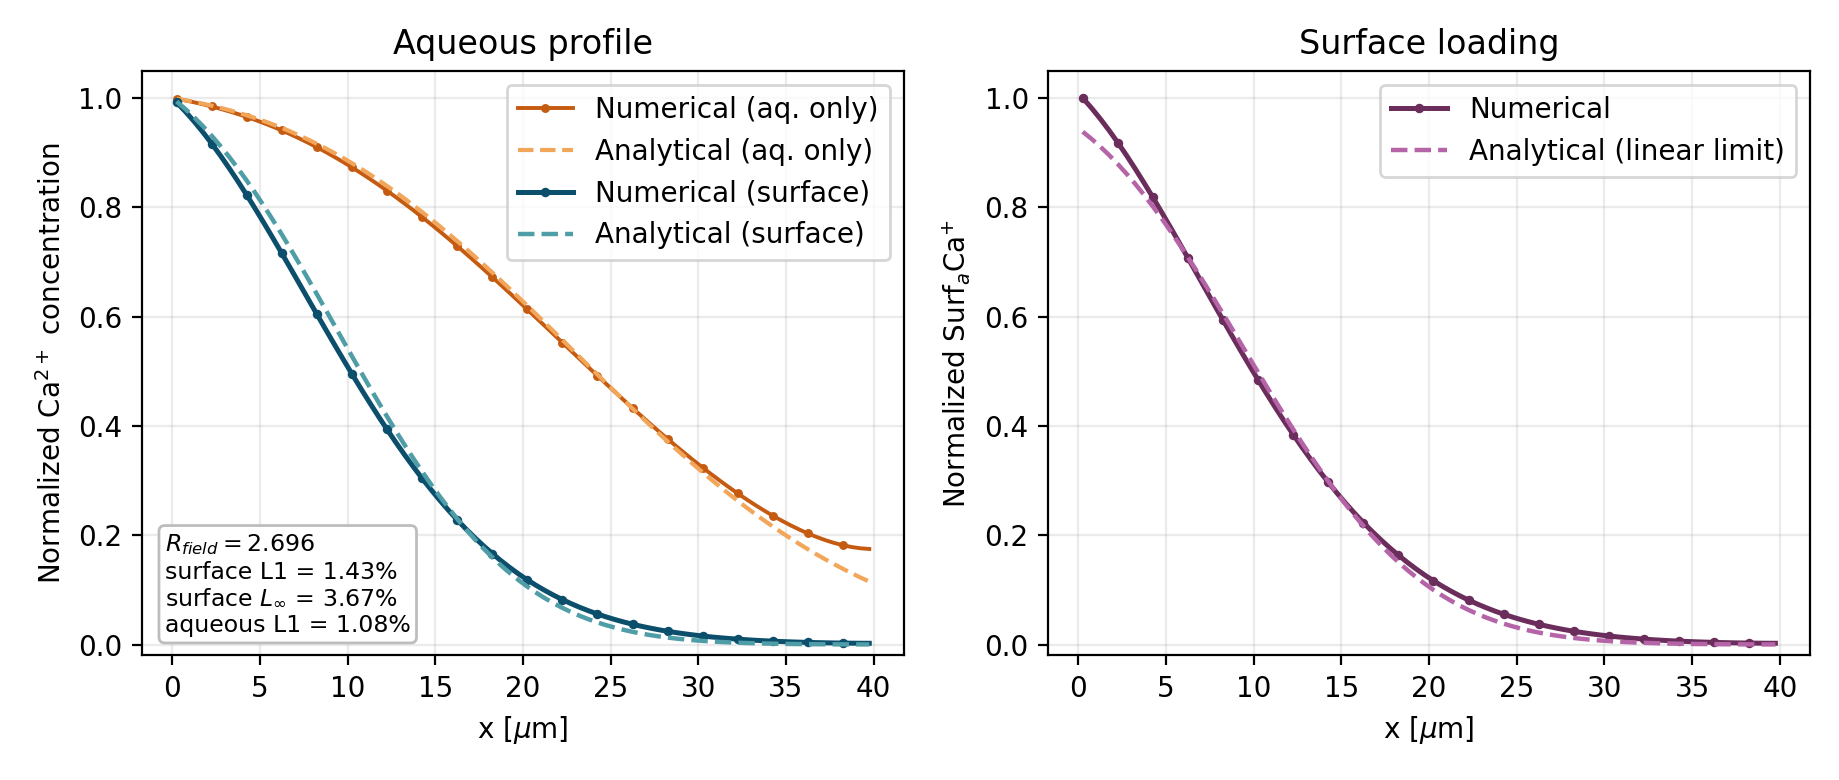
\includegraphics[width=0.9\linewidth]{figures/png/fig01_1d_retardation.png}
    \caption{1D analytical retardation benchmark: spatial profiles at $t = 10$.
    Left: normalized aqueous Ca$^{2+}$ profiles for the aqueous-only and
    surface-enabled runs, compared against their matching cell-averaged
    advection-diffusion analytical solutions. Right: normalized surface loading
    compared against the cell-averaged linear-equilibrium analytical limit
    constructed from the calibrated field-level $K_{s,\mathrm{field}}$.}
    \label{fig:1DRetardation}
\end{figure}

\begin{figure}[htbp]
    \centering
    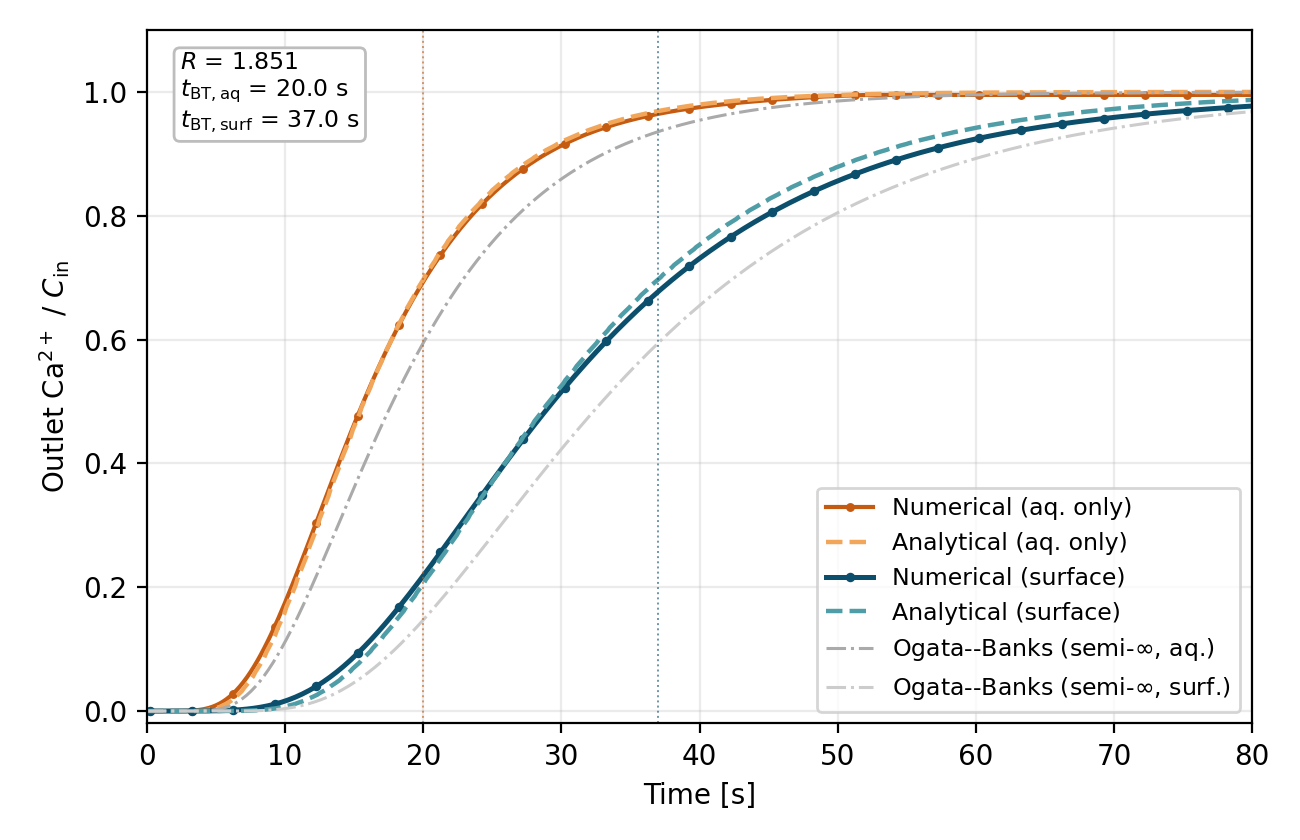
\includegraphics[width=0.9\linewidth]{figures/png/fig06_1d_breakthrough.png}
    \caption{1D outlet breakthrough curves. Symbols show the outlet-patch
    area-averaged Ca$^{2+}$ normalised by the inlet concentration $C_{\mathrm{in}}$
    for the aqueous-only run (circles) and the surface-enabled run (squares).
    Dashed lines are the finite-domain analytical reference; dash-dot lines are
    the semi-infinite Ogata--Banks solution~\citep{ogata1961solution}.
    Vertical dotted lines mark the advective breakthrough times
    $t_{\mathrm{BT}} = L\theta/U$ (aqueous-only) and
    $t_{\mathrm{BT}} = L\theta R_{\mathrm{field}}/U$ (surface-enabled).}
    \label{fig:1DBreakthrough}
\end{figure}

\subsection{Closed-System Batch Balance}

The chemistry--transport interface is verified against the exact
species-inventory identity for a closed batch domain (no inflow or outflow,
$\mathbf{u} = 0$).
Conservation of the total field-level Ca$^{2+}$ inventory requires
\begin{equation}
    \mathcal{M} \;=\; \theta\,C + a_{\mathrm{surf}}\,\Gamma \;=\; \mathrm{const},
    \label{eq:closedBalance}
\end{equation}
where $C$ is the aqueous concentration, $\Gamma$ is the surface loading, and
$\theta$ and $a_{\mathrm{surf}}$ are the same domain-averaged porosity and
surface-area density as in the 1D transport benchmark.
In the linear dilute limit, Eq.~\eqref{eq:closedBalance} gives the equilibrium
partition
\begin{equation}
    C_{\mathrm{eq}} = \frac{\theta\,C_0}{\theta + a_{\mathrm{surf}}\,K_{s,\mathrm{field}}},
    \label{eq:batchEquil}
\end{equation}
which is equivalent to $C_0 / (1 + a_{\mathrm{surf}}\,K_{s,\mathrm{field}}/\theta)$.

Two tests are run on the 80\,\texttimes\,1\,\texttimes\,1 mesh with
$\theta = 0.5$ and $a_{\mathrm{surf}} = 10^5\,\mathrm{m^{-1}}$ using the same
Ca$^{2+}$--\texttt{Surf\_a} surface chemistry as in Section~\ref{sec:1D}.
In the \emph{adsorption} test the domain is initialised with a fully aqueous
inventory ($\theta\,C_0 = 4.49 \times 10^{-4}\,\mathrm{mol\,m^{-3}}$,
$\Gamma_0 \approx 0$) and the batch-equilibration solver brings the system to
equilibrium in a single PHREEQC call; Ca$^{2+}$ partitions from the pore
fluid onto the surface.
In the \emph{desorption} test the inventory is loaded entirely onto the
surface ($\Gamma_0 > 0$, $C_0 \approx 0$) and equilibrium is re-established;
Ca$^{2+}$ desorbs back into the pore fluid.
The relative inventory drift
$|\mathcal{M}_{\mathrm{end}} - \mathcal{M}_{\mathrm{start}}| / \mathcal{M}_{\mathrm{start}}$
is $1.2 \times 10^{-7}$ for adsorption and $7.2 \times 10^{-7}$ for
desorption, both well below the \mbox{$10^{-6}$} tolerance.
This confirms that the chemistry--transport interface conserves the total
field-level Ca$^{2+}$ inventory to the PHREEQC convergence level in both
the adsorption and desorption directions.

\subsection{Validation Summary}\label{sec:valSummary}

In addition to the 1D analytical benchmark and the closed-system batch
balance, the solver has been verified against a set of controlled numerical
baselines on the same domain.
The aqueous-only and \mbox{$a_{\mathrm{surf}} = 0$} reductions confirm that
the solver degrades correctly to standard advection--diffusion transport when
surface chemistry is absent.
Closed-system adsorption--desorption cycles confirm that the total
aqueous-plus-surface Ca$^{2+}$ inventory is conserved at relative drifts of
$1.2 \times 10^{-7}$ and $7.2 \times 10^{-7}$, demonstrating that the
chemistry--transport interface preserves global species balance to the
PHREEQC convergence level in both directions.
Sensitivity studies on the operator-splitting step size, the physical
timestep, and the mesh resolution quantify the local and bulk drift at
practical settings.
Table~\ref{tab:validationSummary} summarises the key metrics from this
benchmark family.

\begin{table}[htbp]
    \centering
    \caption{Validation summary for the tracked 1D benchmark family.
    ``Splitting'' refers to the operator-splitting (chemistry--transport)
    consistency test; ``Timestep'' and ``Mesh'' are sensitivity studies on
    the fixed 1D benchmark. The performance row reports the fraction of
    wall-clock time spent in PHREEQC across the sensitivity runs.}
    \label{tab:validationSummary}
    \begin{tabular}{lll}
        \toprule
        Check & Metric & Result \\
        \midrule
        Analytical 1D & Surface L1 / total drift & $1.43\%$ / $1.57\%$ \\
        Closed-system (ads./des.) & Inventory drift & $1.2\times10^{-7}$ / $7.2\times10^{-7}$ \\
        Splitting     & Local / bulk drift        & $3$--$4.5\%$ / $<0.6\%$ \\
        Timestep      & Local / bulk drift        & $\approx 3\%$ / $0.25\%$ \\
        Mesh          & Front / total drift       & $2.5\times 10^{-7}$ / $0.37\%$ \\
        Performance   & Surface chemistry fraction & $36$--$55\%$ \\
        \bottomrule
    \end{tabular}
\end{table}

A consistent pattern emerges across the sensitivity studies: local
(cell-level) drift reaches $3$--$4.5\%$ while bulk (volume-integrated) drift
stays below $0.6\%$.
This disparity indicates that operator-splitting and timestep errors are
concentrated near the chemical front and cancel almost completely at the domain
level, so global conservation properties are preserved even where local
truncation errors are non-negligible.
The near-zero front-position drift ($2.5 \times 10^{-7}$) from the mesh study
confirms that the retardation-front position is not systematically biased by
mesh resolution.
The surface chemistry fraction of $36$--$55\%$ of wall-clock time reflects the
per-cell cost of the PHREEQC equilibrium solve for a dilute two-ion system;
the same per-cell cost governs chemistry overhead in the 3D image-based cases,
where it scales with the number of mobile cells rather than with domain topology.

\subsection{Two-Scale Upscaling Validation}\label{sec:twoScaleValidation}

The upscaled formulation is tested directly against a fully resolved
lithium-sorption calculation on the same long micromodel geometry. The fully
resolved reference retains binary pore and grain cells, whereas the DBS case
represents the unresolved pore structure through its coarse-cell properties and
internal reactive surface area. Both cases use the same inlet chemistry and are
compared at matched P\'{e}clet number and normalized advective distance $x/L$.
This removes the difference in physical travel time caused by the separately
calibrated flow fields.

The fully resolved production resolution was selected after categorical
downsampling tests at $5$, $10$, and $15~\mu$m. Categorical majority voting was
used throughout: no pore/grain cell was formed by averaging to an intermediate
porosity. The $5~\mu$m image was retained because it preserves the streamwise
pore connectivity and the pore--grain interfaces on which sorption occurs;
coarser images gave increasing local Li-field differences even where bulk
porosity, permeability, and reactive area remained similar.

Figure~\ref{fig:twoScaleErrorPe} compares aqueous and sorbed Li at
$x/L=0.125$ for $\mathrm{Pe}=0.1$, $1$, $3$, and $10$. The acceptance limits
were $5\%$ absolute inventory difference, $10\%$ normalized streamwise-profile
L1 error, and $0.1$ map dissimilarity. Across the sweep, the largest aqueous
and sorbed inventory differences are $2.15\%$ and $1.83\%$, respectively; the
largest profile errors are $2.09\%$ and $5.19\%$; and every map dissimilarity
is below $8.0\times10^{-4}$. All four cases therefore pass the predefined
criteria. The error does not grow systematically with P\'{e}clet number, and no
breakdown of the upscaling is observed by $\mathrm{Pe}=10$ for this geometry.

\begin{figure}[htbp]
    \centering
    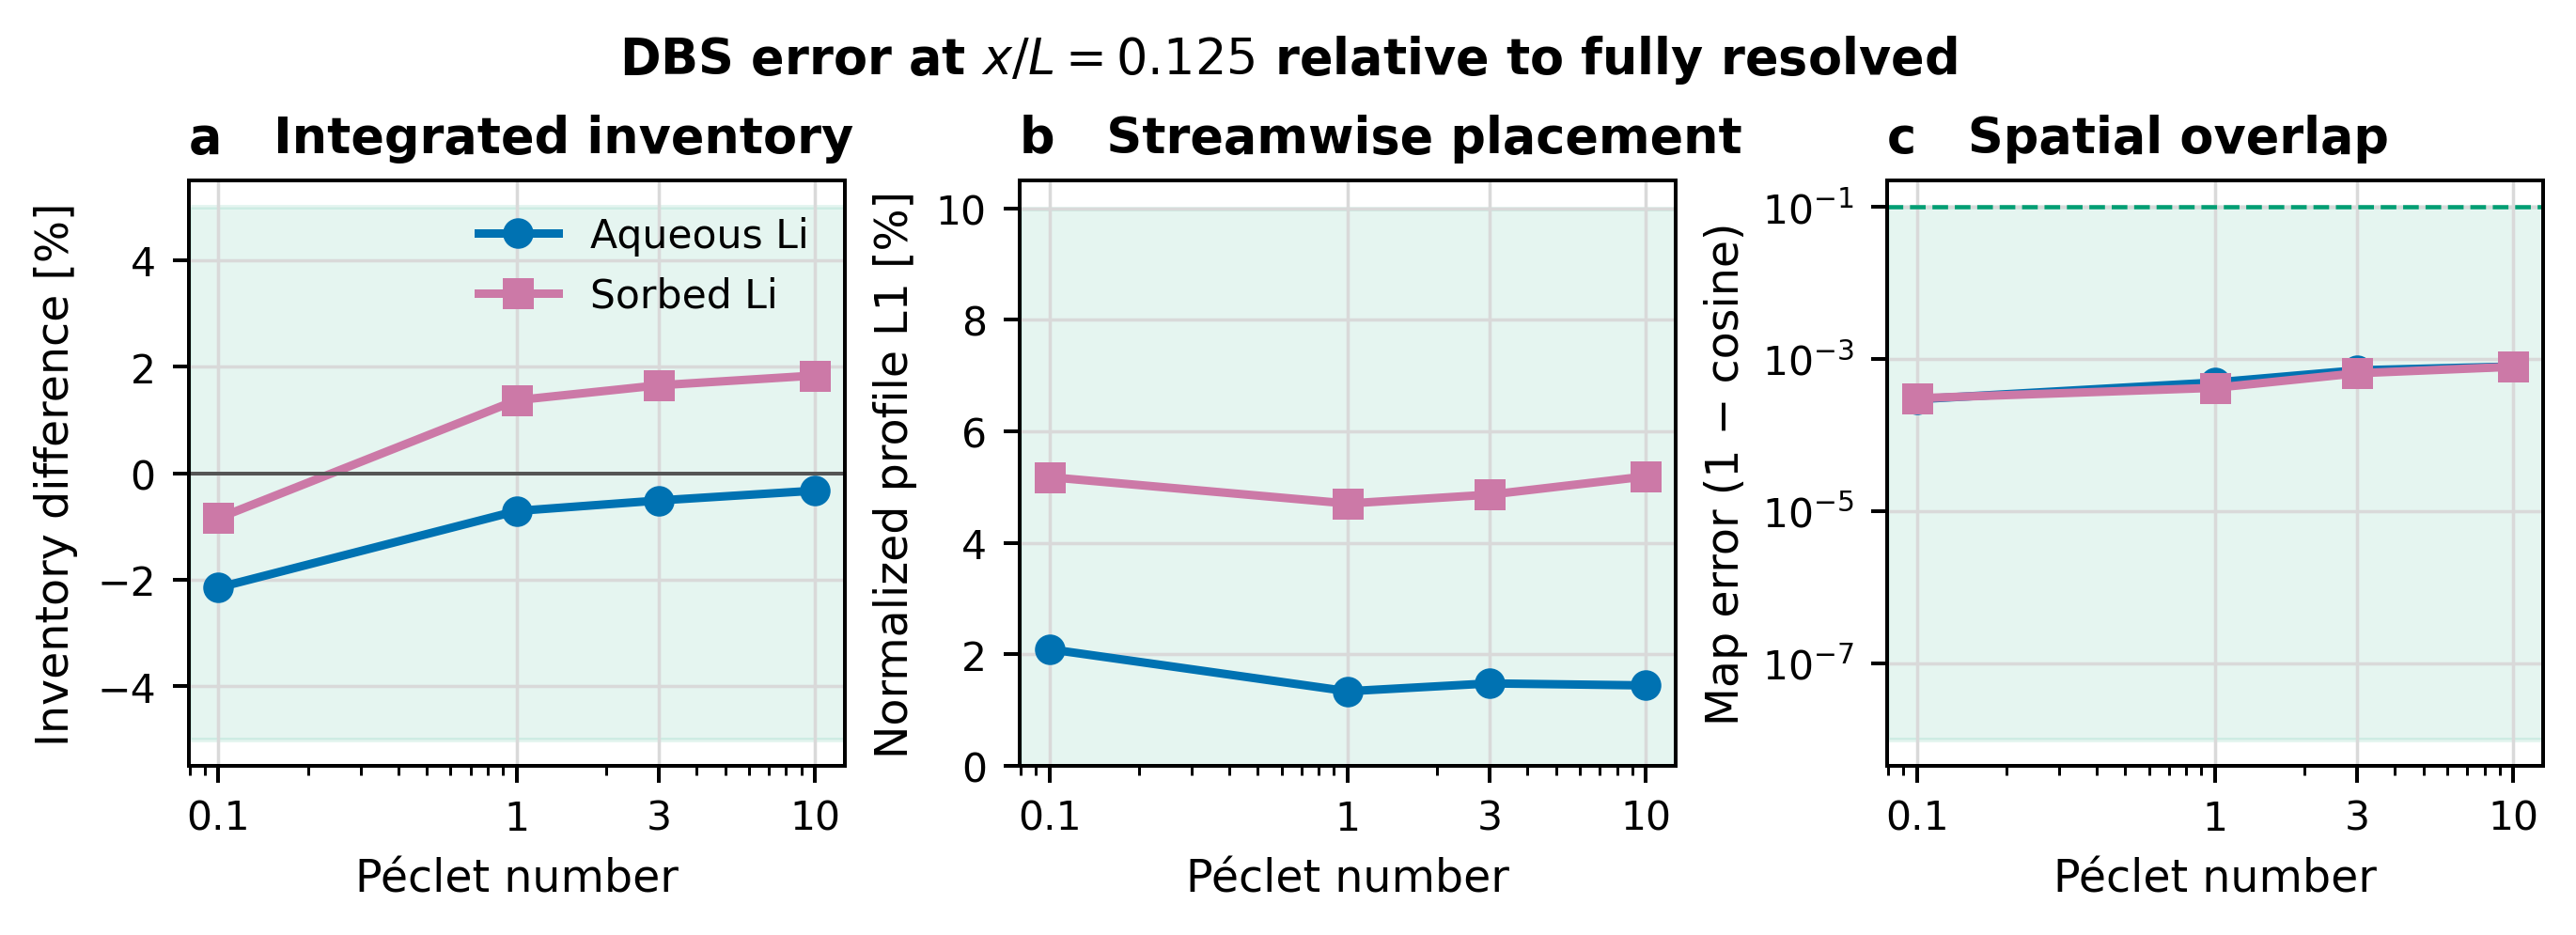
\includegraphics[width=\linewidth]{figures/png/fig09_two_scale_error_vs_peclet.png}
    \caption{DBS-upscaled error relative to the fully resolved lithium-sorption
    reference at matched $x/L=0.125$. (a)~Signed differences in integrated
    aqueous and sorbed Li inventory. (b)~Normalized L1 errors of the
    streamwise profiles. (c)~Map dissimilarity, defined as one minus cosine
    similarity. Green shading marks the predefined acceptance region in each
    panel.}
    \label{fig:twoScaleErrorPe}
\end{figure}

Figure~\ref{fig:twoScalePe1Fields} shows the fields later in the Pe=1 run, at
$x/L=0.625$. The resolved result is plotted on its native $5~\mu$m grid with
grain cells masked rather than spatially averaged. The pore-scale aqueous plume
and sorbed-Li pattern remain visible, while the DBS fields show the corresponding
coarse representation. Their front positions and large-scale plume shapes are
consistent despite the deliberately different local descriptions.

\begin{figure}[htbp]
    \centering
    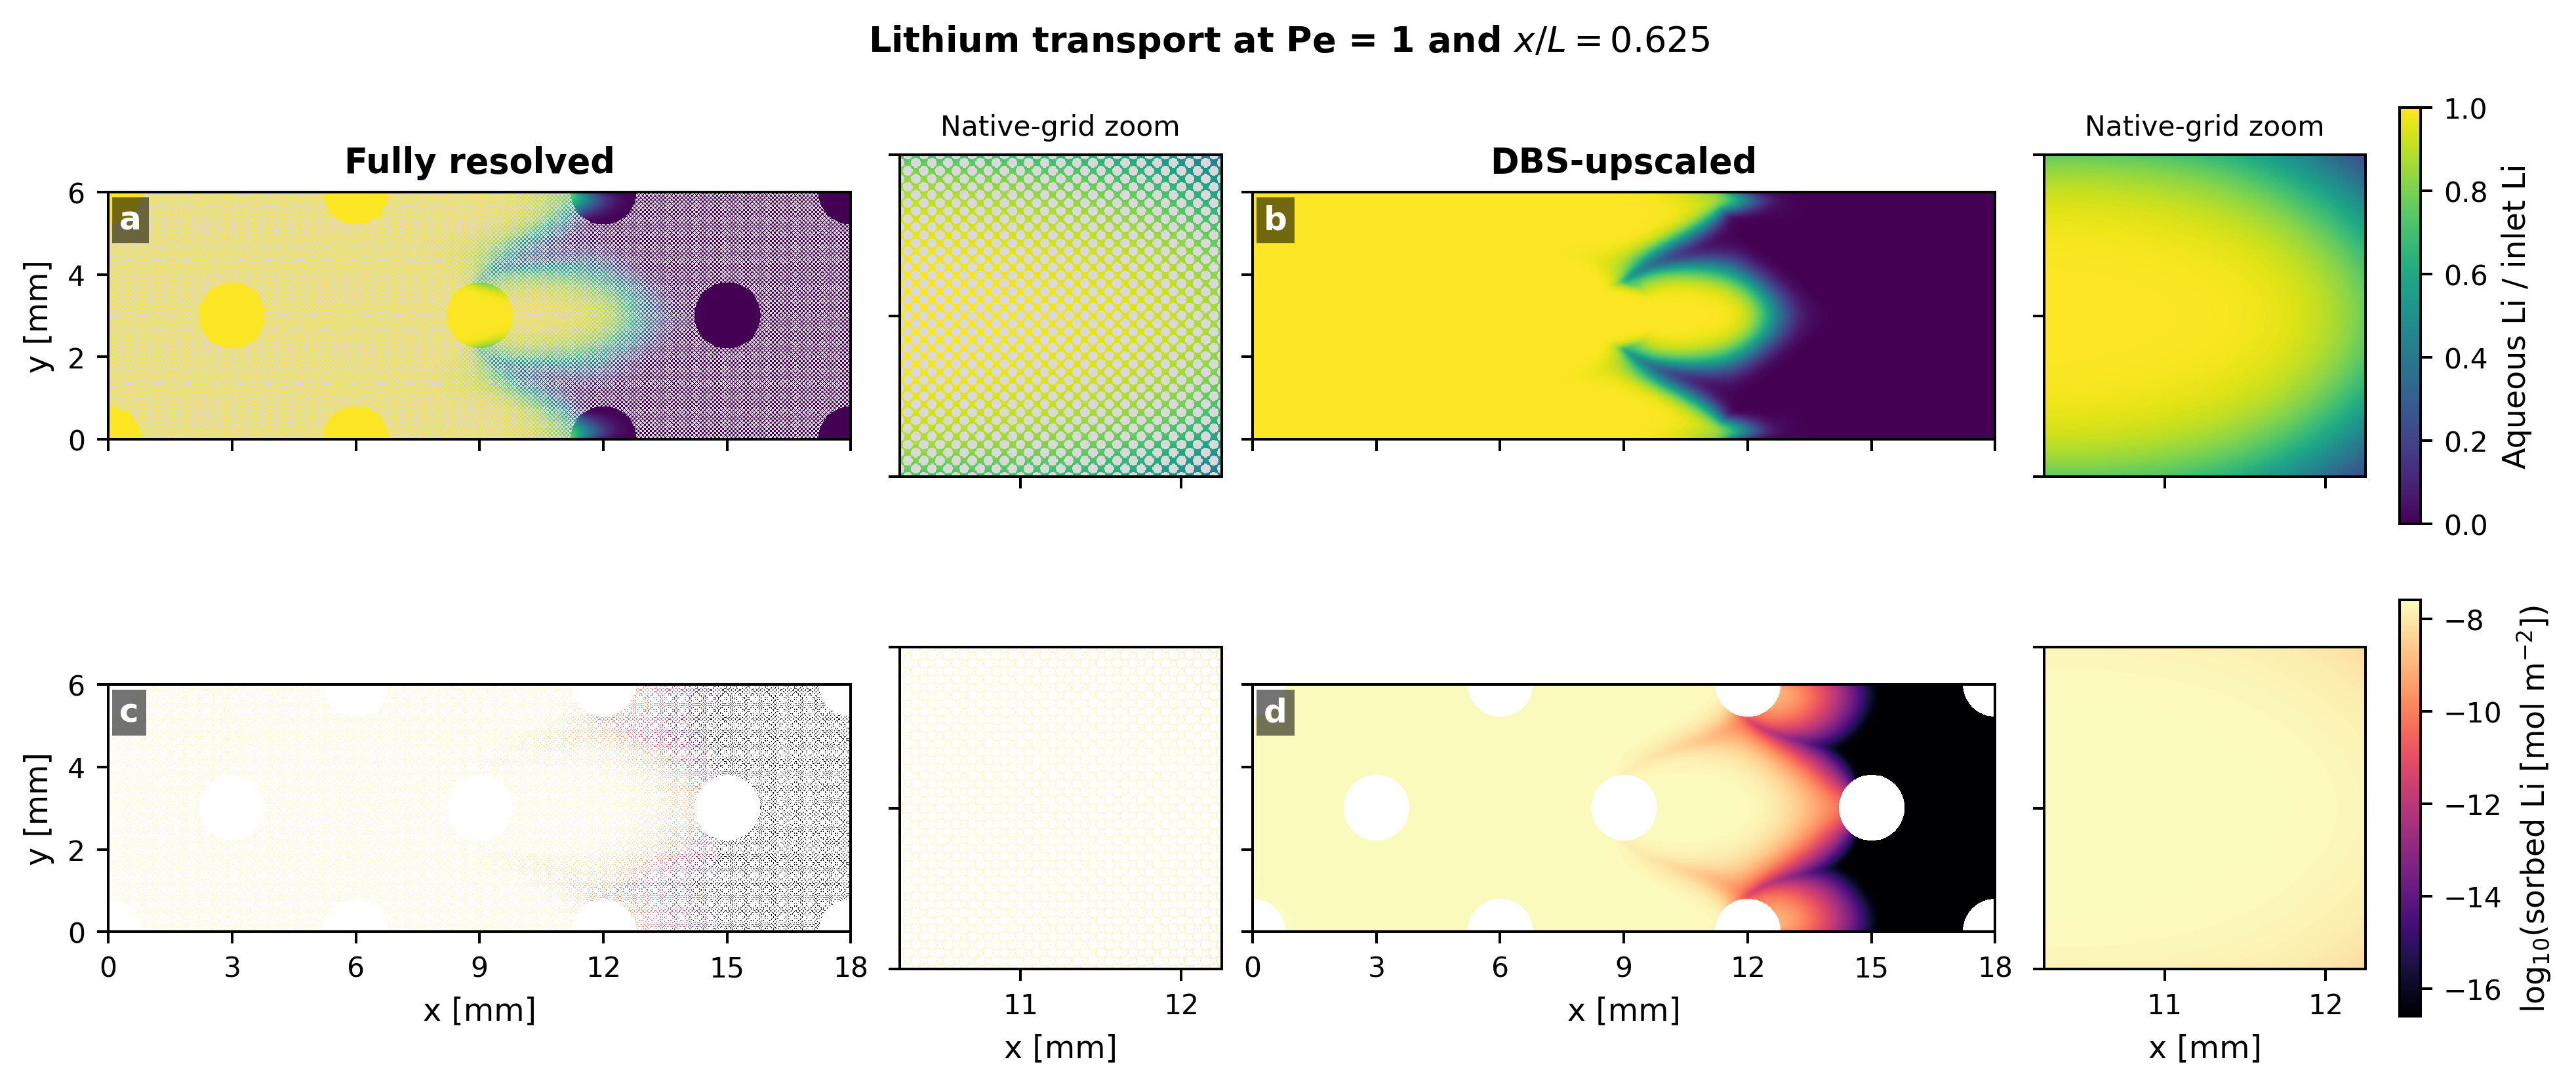
\includegraphics[width=\linewidth]{figures/png/fig10_two_scale_pe1_fields.png}
    \caption{Lithium fields at $\mathrm{Pe}=1$ and matched $x/L=0.625$.
    (a,b)~Aqueous Li normalized by the inlet concentration for the fully
    resolved and DBS-upscaled cases. (c,d)~Corresponding sorbed Li on a shared
    logarithmic scale. The inset panels show the native computational grids;
    the fully resolved pore/grain image is masked, not averaged.}
    \label{fig:twoScalePe1Fields}
\end{figure}

\section{Image-Based Applications}

All applications use $\theta_{\mathrm{mask}}=10^{-3}$ and fixed
$a_{\mathrm{surf}}^{\mathrm{interface}}+a_{\mathrm{surf}}^{\mathrm{intrinsic}}$.
Online Resource~1 provides image, grid, transport, surface-reaction,
concentration, runtime, and MPI specifications for result-supporting cases.

\subsection{Pb$^{2+}$ Uptake in a Two-Dimensional Fracture Network}

The \nolinkurl{4StraightFractures} image contains microporous matrix and open
fractures on a $250\times250\times1$ computational grid. Pb$^{2+}$ enters at
$10^{-3}$~mol\,L$^{-1}$ and equilibrates with strong and weak
Dzombak--Morel HFO sites \citep{dzombak1990surface}. The reactive-area field
combines the reconstructed matrix--fracture interface with
$10^5$~m$^{-1}$ of intrinsic area in the matrix, whose end-member porosity is
$0.4$.

At $t=20000$~s, dissolved Pb$^{2+}$ preferentially follows the connected
fractures while strong-site occupancy extends into the adjacent microporous
matrix (Figure~\ref{fig:2DFractures}). Uptake is greatest near the inlet and
fracture intersections, where advective delivery and matrix area coincide.
The result illustrates the central scale separation: open cells control rapid
delivery, whereas unresolved matrix area controls much of the adsorbed
inventory.

The paired fields distinguish transport access from sorption capacity. The
dissolved field follows the connected fracture network because those cells
carry the rapid flow paths. Strong-site occupancy persists in matrix cells
adjacent to the fractures because the matrix retains mobile water and the
specified intrinsic area. Thus the spatial pattern is not interpreted as a
direct image of velocity: it reflects the overlap of delivered Pb$^{2+}$,
accessible microporous water, and local HFO capacity.

\begin{figure}[htbp]
    \centering
    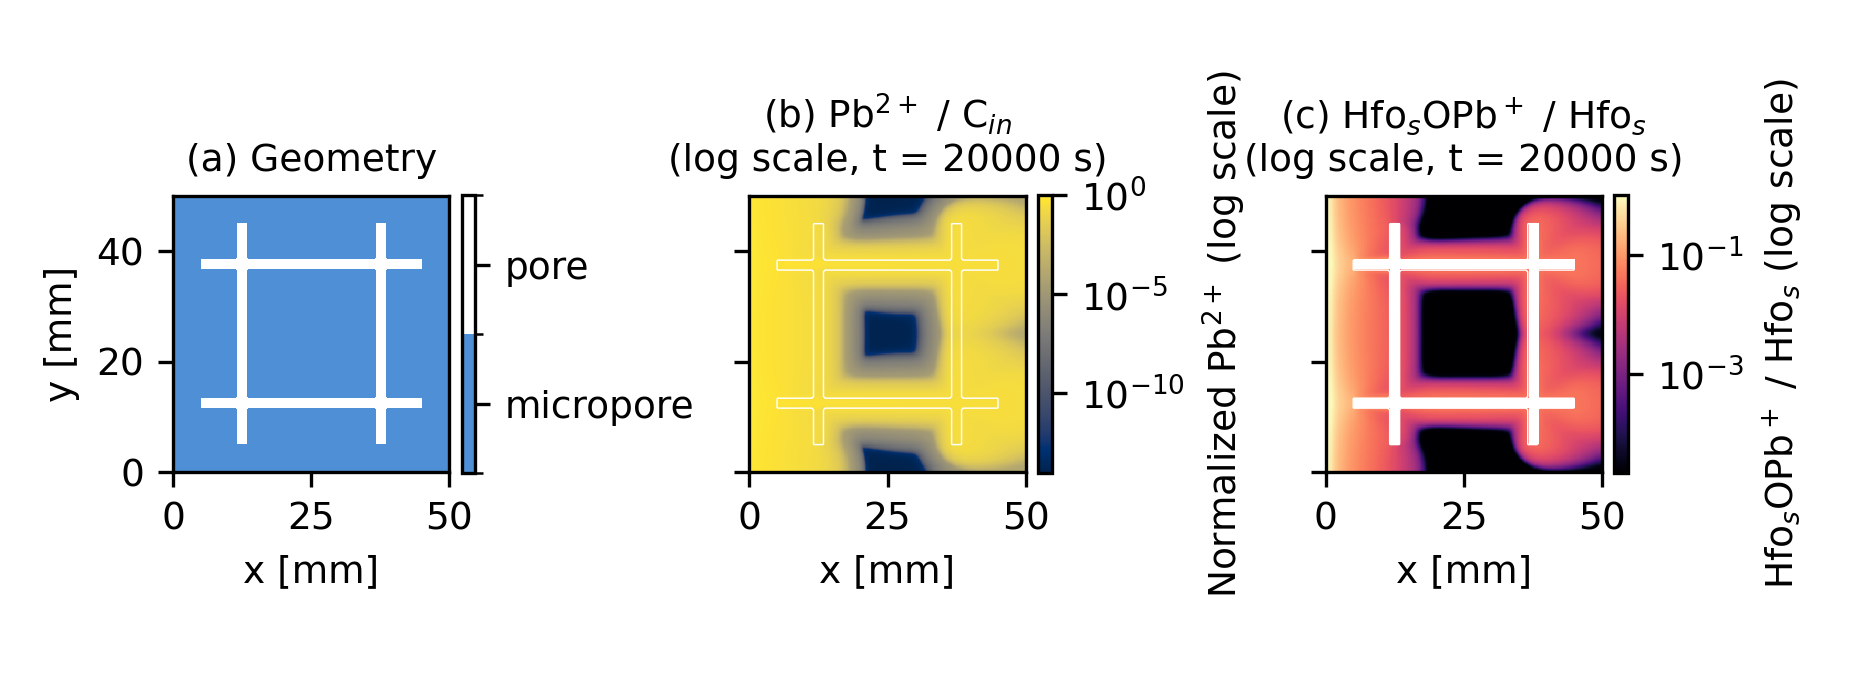
\includegraphics[width=0.82\linewidth]{figures/png/fig02_2d_fractures.png}
    \caption{Pb$^{2+}$ transport and HFO occupancy at $t=20000$~s. From left:
    segmented fracture geometry, dissolved $\mathrm{Pb}^{2+}/C_{\mathrm{in}}$
    with logarithmic colour normalisation, and strong-site occupancy with
    logarithmic colour normalisation. Zero-area cells are masked in the
    occupancy panel.}
    \label{fig:2DFractures}
\end{figure}

\subsection{Sr$^{2+}$/Ca$^{2+}$ Exchange in Estaillades Limestone}

The large application uses a $500^3$ three-phase Estaillades image with
$4~\mu$m voxels \citep{menke2021upscaling}. Open pore, micropore, and solid
labels are represented at native resolution. Micropores carry $\theta=0.4$
and intrinsic area $10^5$~m$^{-1}$. A $10^{-4}$~mol\,L$^{-1}$ Sr$^{2+}$
inlet displaces an initially equilibrated $10^{-3}$~mol\,L$^{-1}$ Ca$^{2+}$
solution from \texttt{Surf\_a} sites; the Sr reaction has the slightly larger
equilibrium constant ($\log K=-5.5$ versus $-5.85$ for Ca).

The image produces chromatographic exchange rather than single-species
retardation. Sr$^{2+}$ adsorption advances behind a Ca$^{2+}$ desorption wave,
and loading follows the connected reactive microporosity
(Figure~\ref{fig:3DEstaillades}). Across the saved checkpoints from 0 to
120~s, the porosity-weighted mean Sr$^{2+}$ concentration rises to $0.865$
$C_{\mathrm{in}}$, while Ca$^{2+}$ falls from $1.000$ to $0.095$
$C_{\mathrm{init}}$. Surface-area-weighted \texttt{Surf\_aSr+} increases
monotonically as \texttt{Surf\_aCa+} decreases
(Figure~\ref{fig:EstailladesTemporal}); the signed changes are referenced to
$t=0$ and divided by the largest absolute change across both surface species
and all plotted times. This directly identifies replacement of
resident Ca by invading Sr.

The temporal and spatial views provide complementary evidence for this
interpretation. The volume rendering shows where the invading dissolved Sr and
its surface loading occur in the connected image, whereas the weighted time
series shows the opposing changes in the Sr and Ca inventories. The Ca decrease
is therefore associated with competitive displacement from the fixed surface
state, rather than being inferred solely from the aqueous front. These
application results illustrate the consequence of representing the internal
microporous area as capacity; they do not independently determine its physical
magnitude.

\begin{figure}[htbp]
    \centering
    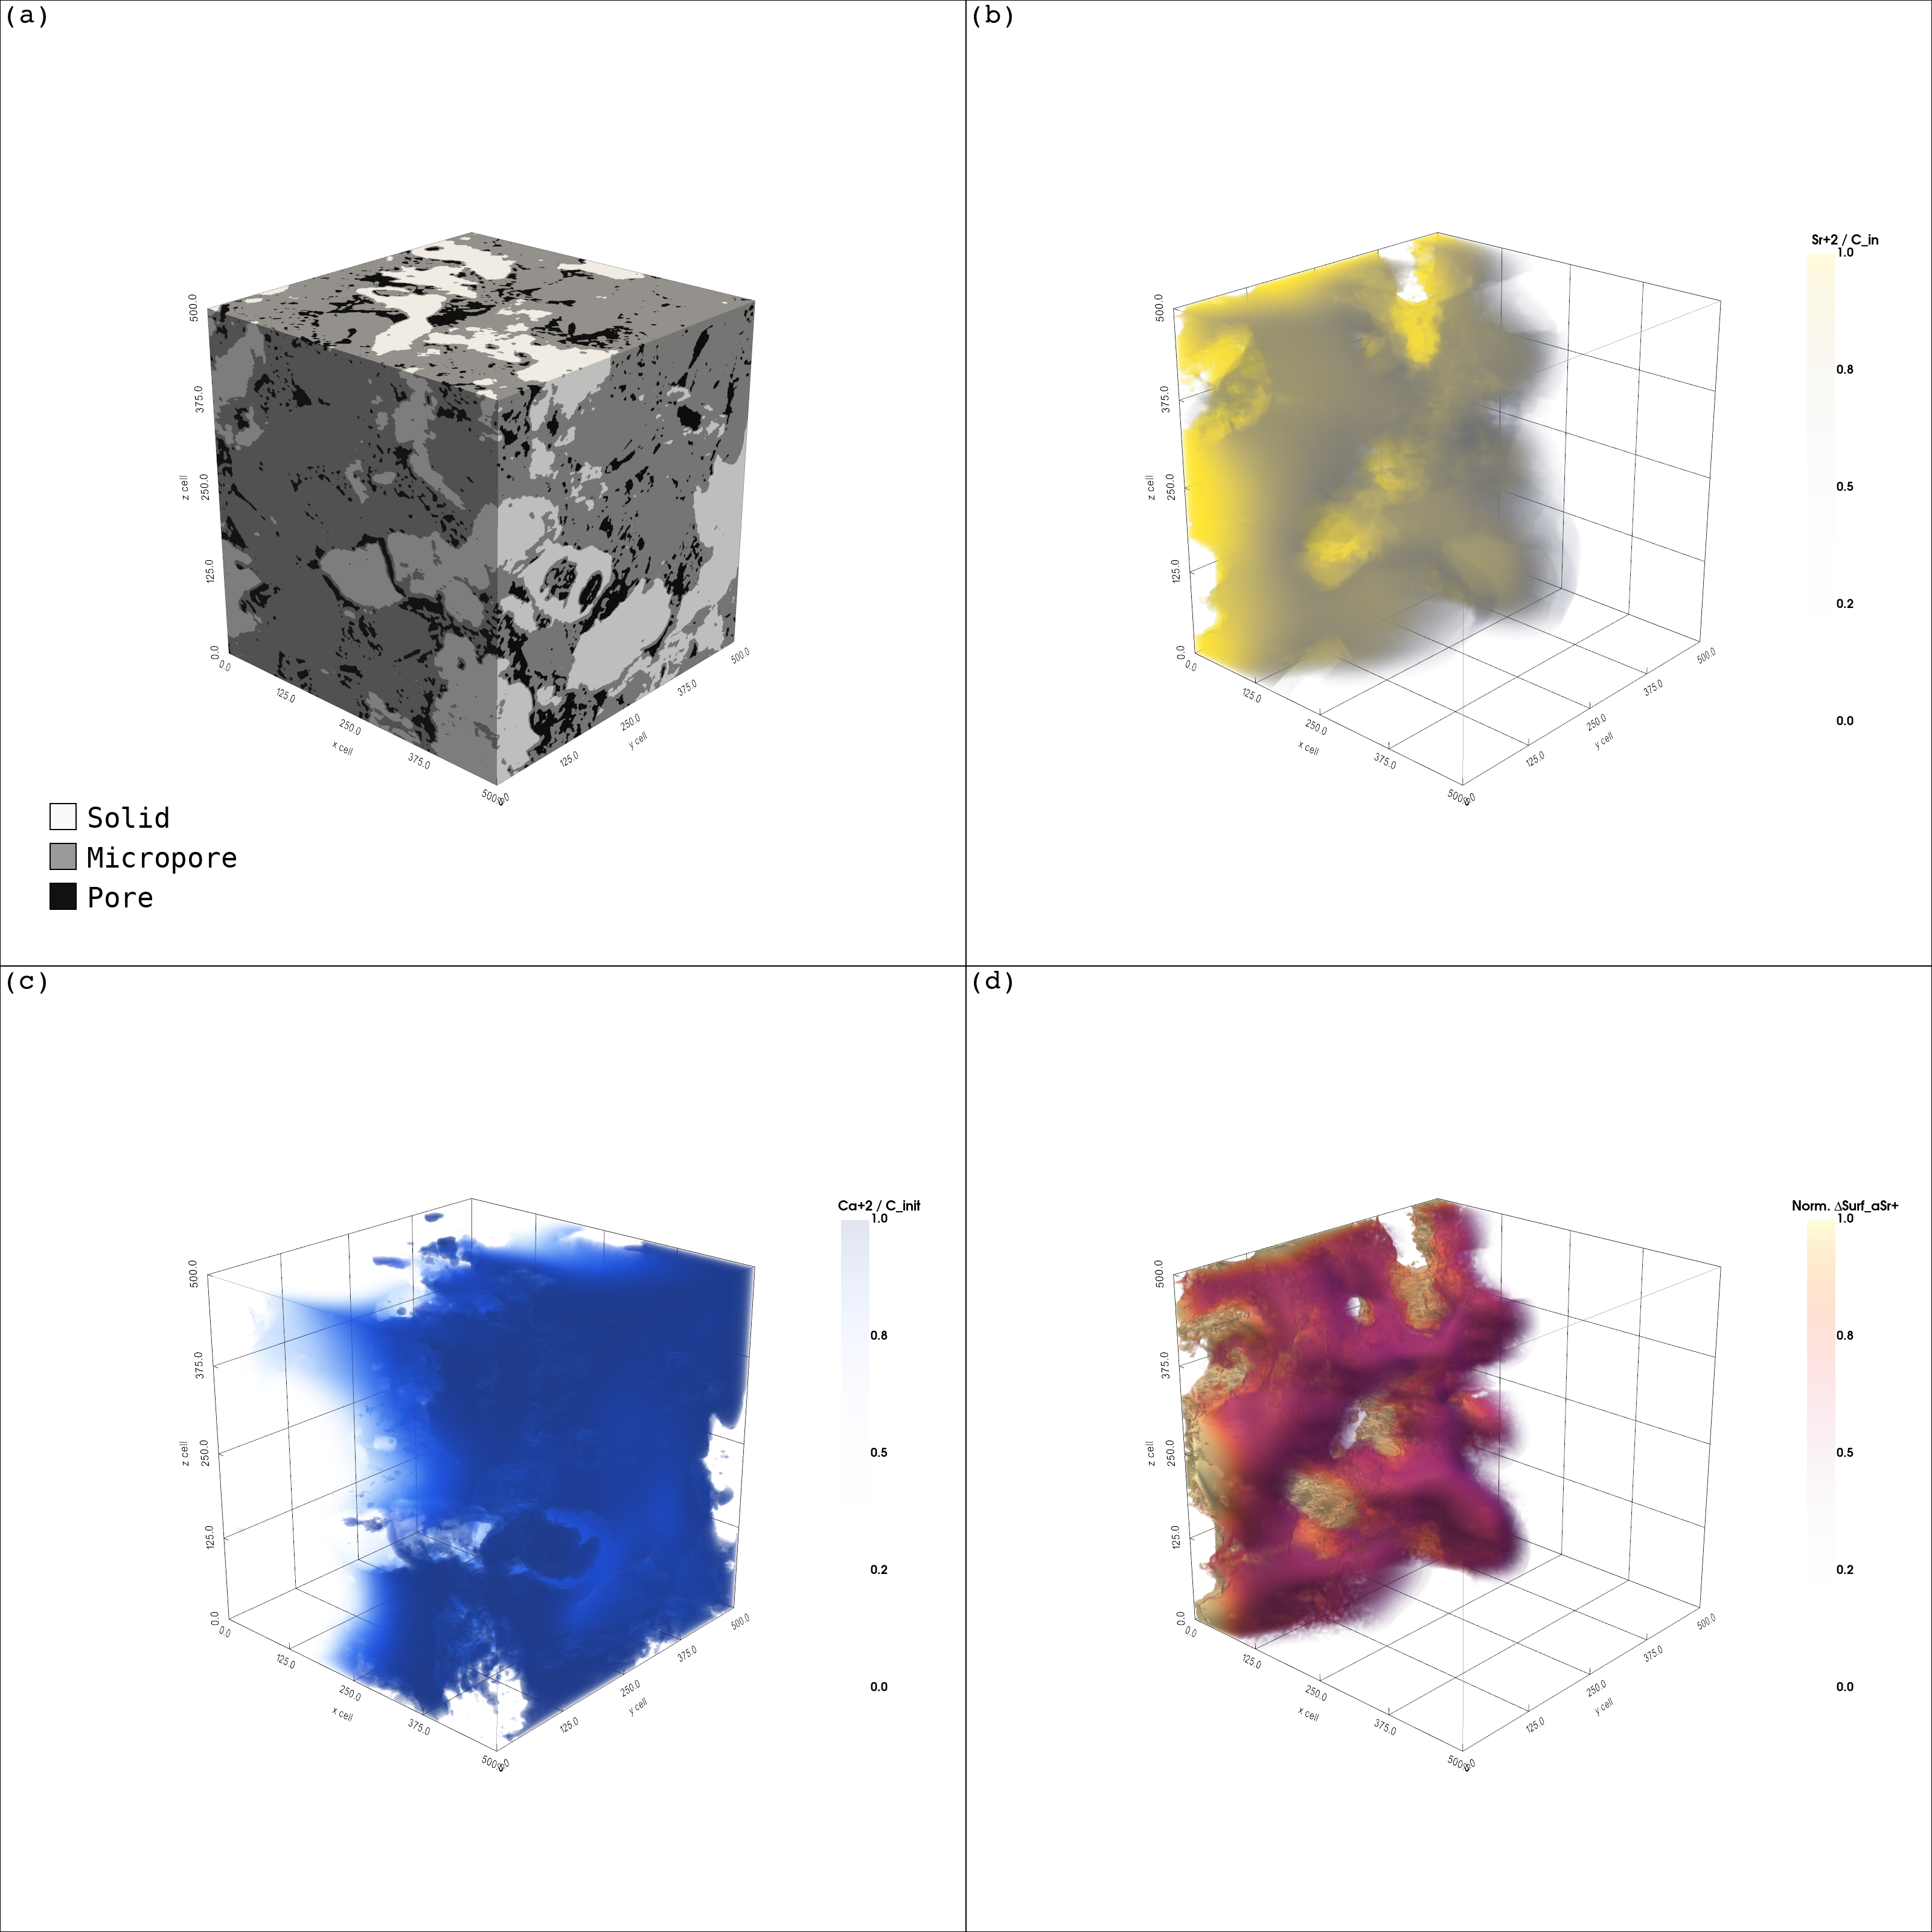
\includegraphics[width=\linewidth]{figures/png/fig04_3d_estaillades.png}
    \caption{Estaillades exchange at $t=40$~s. Panels show the segmented
    geometry, dissolved Sr$^{2+}/C_{\mathrm{in}}$ and
    Ca$^{2+}/C_{\mathrm{init}}$, and the incremental adsorbed Sr$^{2+}$
    loading relative to $t=0$, normalised by its maximum at 40~s. The plume
    enters from the left and loads the distributed microporous surface.}
    \label{fig:3DEstaillades}
\end{figure}

\begin{figure}[htbp]
    \centering
    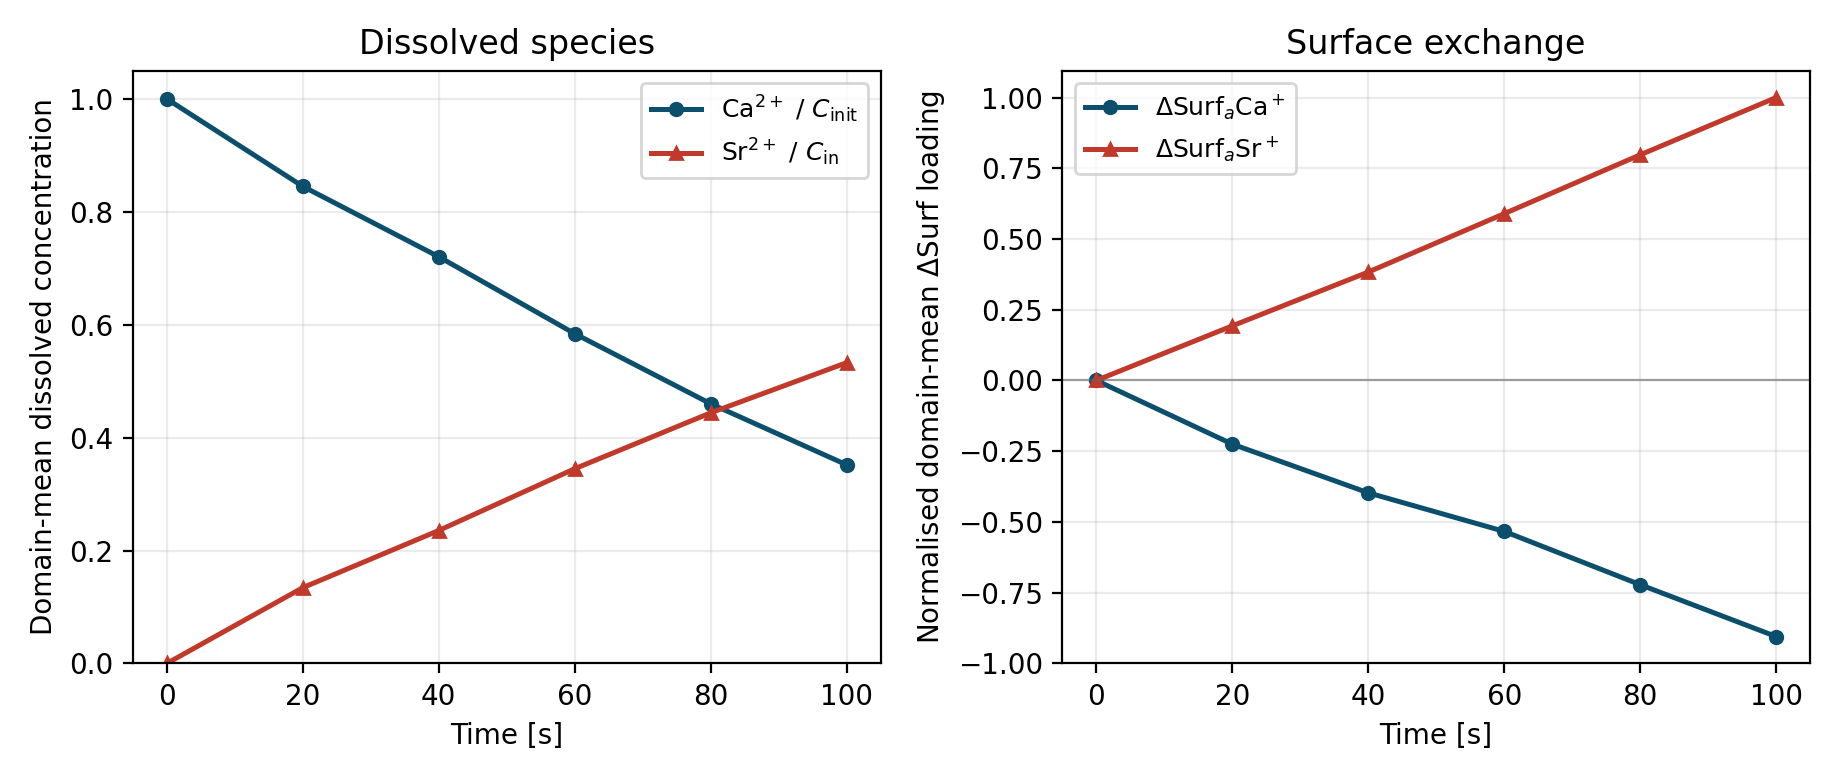
\includegraphics[width=0.86\linewidth]{figures/png/fig08_estaillades_temporal.png}
    \caption{Estaillades exchange from 0 to 120~s. Porosity-weighted dissolved
    Ca$^{2+}$ and Sr$^{2+}$ (left) are paired with signed changes in
    surface-area-weighted adsorbed amounts (right). Each surface change is its
    value minus that at $t=0$, divided by the largest absolute change across
    both species and all plotted times, showing Sr invasion and Ca displacement
    in both inventories.}
    \label{fig:EstailladesTemporal}
\end{figure}

\section{Discussion}

\subsection{Formulation Choices and Conservative Structure}

The central modelling choice in this work is to use one fixed porosity field,
$\theta$, in the finite-volume transport equation and in the PHREEQC cell
volumes alike, which keeps aqueous accumulation, transport, and equilibrium
chemistry on the same volumetric basis. The reactive surface is prescribed
independently through the explicit cell field $a_{\mathrm{surf}}$, so the
chemical storage volume and the amount of reactive surface remain separately
defined material properties.

This approach extends earlier micro-continuum reactive transport formulations
to the case where the reactive surface area is an unresolved cell property
rather than an explicitly meshed boundary. In existing pore-scale DBS solvers,
including \nolinkurl{porousMedia4Foam} and earlier GeoChemFoam solvers,
reactive uptake is typically imposed as a flux condition on the diffuse
fluid-solid interface. This requires the reactive surface to coincide with the resolved image voxel
boundary, which is a good approximation when the dominant reactive area lies at
the contact between macropore and grain. In multi-scale carbonate images the
microporous phase holds a large internal reactive area that lies inside the
coarse cell rather than on its boundary. The cell-based formulation carries
that area as an intrinsic volumetric density
$a_{\mathrm{surf}}^{\mathrm{intrinsic}}$, scaled by the local phase fraction
and passed to PHREEQC as a cell-level property.

Conservation is therefore enforced at the cell level rather than through a face
flux. The combined inventory $M = \theta C + a_{\mathrm{surf}}\Gamma$ is updated
locally by PHREEQC at each timestep, and the aqueous transport step is
conservative in the standard finite-volume sense, so the only mass-balance
error is the splitting error of the coupling itself. The 1D analytical
benchmark measures that error directly.

\subsection{Geometric Scalability}

Because the validation ladder separates conservative coupling, surface-area
geometry, and microporosity, each error can be attributed to the layer that
produced it: the coupling to within $1.2\%$ in bulk inventory against the
analytical retardation factor, the interface-area construction to sub-percent
accuracy against analytic spheres and posts, and the intrinsic micropore
density only in the cases that use it.

The transition from 2D to 3D introduces qualitatively different transport paths
and surface-loading distributions. In the 2D case, open fractures provide
preferential pathways for dissolved Pb$^{2+}$, while strong-site Pb occupancy
varies across the surrounding microporous matrix and is enhanced near the inlet
and fracture intersections. In the 3D cases, the tortuosity of the
pore network produces a more dispersed front and a more heterogeneous
surface-loading pattern. This spatial heterogeneity in surface uptake controls the effective retardation
factor seen at the continuum scale, and following it requires a simulation that
resolves the local connectivity of the image.

The direct resolved-to-DBS comparison shows that the coarse representation also
preserves the bulk transport and sorption response across $Pe = 0.1$ to $10$,
with inventory differences below $0.9\%$ and profile errors below $5.8\%$, both
growing with $Pe$ across the sweep. That growth sets the direction of the
remaining uncertainty: higher $Pe$, different connectivity, or sharper kinetic
fronts may expose an upscaling failure that this range does not.

\subsection{Computational Cost and Scaling}

PHREEQC is called once per active cell per timestep, with a full speciation
and surface-equilibration calculation for each cell. The chemistry overhead
therefore depends primarily on the number of active cells, the geochemical
system, and the frequency of the chemistry call. For larger grids or more complex geochemical systems, masking near-solid cells
out of the PhreeqcRM mapping (here at
$\theta \le \theta_{\mathrm{mask}} = 10^{-3}$) is the main lever on that cost.
The threshold is held fixed across all examples here, and its influence on
accuracy and cost deserves a dedicated sensitivity study.

\subsection{Limitations and Future Work}

The intrinsic micropore surface density $a_{\mathrm{surf}}^{\mathrm{intrinsic}}$
is a user input per image phase rather than a quantity inferred from the
segmented image, so it must be estimated from complementary measurements such
as nitrogen BET adsorption, mercury intrusion porosimetry, or secondary image
analysis at a finer resolution \citep{noiriel2009changes}. Once the
surface-area construction has been validated, this density is the leading
physical uncertainty in microporous applications, because the accuracy of the
predicted uptake follows directly from how well it represents the internal
reactive area. Linking image-derived phase fractions to measured or computed
internal surface-area densities, and quantifying the sensitivity to that input,
is the next step.

The upscaled DBS treatment assumes that unresolved matrix properties can be
carried as local cell-averaged quantities. This holds when diffusive exchange
between the resolved pore space and the unresolved matrix is fast compared with
the advective residence time, so that the intrinsic surface area acts as a
locally accessible reactive reservoir. At larger $Pe$, advective bypass and
finite matrix-exchange times leave only part of that area accessible to a
passing concentration front, and the sorption error then carries uncertainty in
the temporal accessibility of the surface as well as in its amount. Local
equilibrium upscaling of an unresolved reactive matrix shares this limitation,
so $Pe$-resolved benchmark comparisons are needed when the method is applied to
strongly advective systems.

Transport and chemistry are coupled by a first-order Lie splitting, which
introduces a splitting error that scales with the timestep and the stiffness of
the reaction terms. For the surface-complexation systems used here, that error
sits within the benchmark agreement reported in Section~\ref{sec:validation},
but it may become significant for faster reactions or stiffer geochemical
systems. A second-order Strang splitting \citep{strang1968construction} is the
natural extension.

Restart depends on the serialised PHREEQC state written with each complete
checkpoint, because the finite-volume \texttt{Surf\_*} fields alone cannot
reconstruct that state. The production $Pe$ sweep restarted from these
checkpoints across several jobs, and moving a run between machines requires the
field data and its matching PHREEQC dump to travel together.

The cases here use a fixed surface area and equilibrium surface complexation,
and cover competitive multi-component chemistry and a Li-selective multi-ion
brine within that scope. Evolving reactive area, mineral dissolution and
precipitation, kinetic surface reactions, and the wider range of mineral
surfaces and aqueous compositions found in natural systems lie outside it.
Extending the model to them will require benchmarks that separate transport
error, surface-area evolution, and reaction-model uncertainty while retaining
cell-level mass-balance checks.

\section{Conclusions}

This work presents a conservative DBS formulation for PHREEQC-coupled reactive
transport with cell-based surface complexation in image-based porous media. The
formulation defines the continuous model, the discrete implementation, and the
validation sequence used to assess the solver across a range of analytical,
image-based, and multi-scale porous-media cases.

The key contribution is a cell-based representation of unresolved reactive
surface area that is consistent with the DBS micro-continuum framework. By
using the physical mobile-water fraction $\theta$ as the accumulation and
chemistry storage variable, rather than the numerical DBS porosity, the method
preserves conservative aqueous transport and well-defined local mass balances
simultaneously. The unresolved micropore surface area is
introduced as an additive intrinsic volumetric density, allowing the method to
represent reactive uptake in image phases where the internal surface area
exceeds what can be recovered from the coarse-cell boundary alone.

The reported results demonstrate that the formulation: (i) reproduces the
dilute analytical retardation limit with sub-percent bulk inventory error;
(ii) produces resolved dissolved and adsorbed fields in
transparent 2D and 3D image-based geometries; and (iii) remains computationally
tractable at application scale, with chemistry representing 36--55\% of the
total wall-clock time for the calcium surface-complexation system studied here,
with cell masking providing an effective cost control for near-solid regions.

The method closes a specific gap in existing DBS reactive transport
capabilities: conservative, unresolved surface complexation in multi-scale
image-based simulations, without requiring the reactive surface to coincide
with an explicitly resolved mesh boundary. This capability is directly relevant
to reactive porous-media problems in which selectivity and surface accessibility
control performance, including contaminant retention, radionuclide migration,
and critical-mineral recovery by sorbent-bearing porous media. The natural
extensions of this work include Strang splitting for reduced
operator-splitting error, better constraints and sensitivity studies for
intrinsic surface-area inputs and masking thresholds, and extensions to
evolving reactive area and kinetic surface chemistry.


\backmatter

\bibliography{references}

\section*{Statements and Declarations}

\textbf{Funding:} This work was supported by the Natural Environment Research
Council (NERC) and Nuclear Waste Services (NWS) through the GeoSAFE grant
(reference NE/Y002504/1). Opinions, findings, conclusions or recommendations
expressed are those of the authors and do not necessarily reflect the views
of NERC or NWS.

\textbf{Competing interests:} The authors have no relevant financial or
non-financial interests to disclose.

\textbf{Ethics approval:} Not applicable.

\textbf{Consent to participate:} Not applicable.

\textbf{Consent for publication:} Not applicable.

\textbf{Availability of data and materials:} The data and materials supporting
this study are available from the corresponding author on reasonable request.

\textbf{Code availability:} The GeoChemFoam 5.2 codebase is publicly available
at \url{https://github.com/GeoChemFoam/GeoChemFoam-5.2}. The solver modifications,
paper-specific cases, simulation scripts, and post-processing code are available
from the corresponding author on reasonable request.

\textbf{Authors' contributions:} \textbf{Hannah P. Menke:} Conceptualisation,
Methodology, Software, Investigation, Formal analysis, Writing -- original
draft, Funding acquisition. \textbf{Julien Maes:} Conceptualisation,
Methodology, Writing -- review \& editing, Funding acquisition.
\textbf{Florian Doster:} Conceptualisation, Writing -- review \& editing,
Funding acquisition.

\end{document}
